
\begin{center}
%    \newcolumntype{P}[1]{>{\centering\arraybackslash}p{#1}}
    \begin{tabular}{ P{2cm} | P{2cm} P{2cm} P{2cm} P{2cm} P{2cm} }
      \small Original nodes &
      \small No. of connections &
      \small Results/ Head &
      \small \phantom{\rule{1.9cm}{1pt}} Queue &
      \small \phantom{\rule{1.9cm}{1pt}} RCM &
      \small \phantom{\rule{1.9cm}{1pt}} New nodes\\
      \hline\normalsize
      1             & 1              & 1          & 5    &7    &1        \\
      2             & 3              & 5          & 3    &4    &2        \\
      3             & 2              & 3          & 2    &8    &3        \\
      4             & 1              & 2          & 6,8  &6    &4        \\
      5             & 2              & 6          & -    &2    &5        \\
      6             & 2              & 8          & -    &3    &6        \\
      7             & 1              & 4          & 7    &5    &7        \\
      8             & 2              & 7          & -    &1    &8        \\
    \end{tabular}
\end{center}
  
  %\vskip 5pt
  \noindent
  Note that the labels of new nodes are the reverse of the elements in the array
  Results.  See below the re-ordered matrix and the adjacency graph (note the
  diagram remains unchanged, but nodes are now relabelled).
  \vskip 5pt
  \noindent
  \begin{table}[H]
    \begin{minipage}[b]{0.50\linewidth}
      \vskip 5pt
      \begin{center}
        $B=
        \begin{bmatrix}
          1 & 1 & 0 & 0 & 0 & 0 & 0 & 0 \\
          1 & 1 & 0 & 0 & 0 & 0 & 0 & 0 \\
          0 & 0 & 1 & 1 & 1 & 0 & 0 & 0 \\
          0 & 0 & 1 & 1 & 1 & 0 & 0 & 0 \\
          0 & 0 & 1 & 1 & 1 & 1 & 0 & 0 \\
          0 & 0 & 0 & 0 & 1 & 1 & 1 & 0 \\
          0 & 0 & 0 & 0 & 0 & 1 & 1 & 1 \\
          0 & 0 & 0 & 0 & 0 & 0 & 1 & 1
        \end{bmatrix}$
      \end{center}
      \vspace{5mm}
    \end{minipage}
    \begin{minipage}[b]{0.49\linewidth}
      \begin{center}
        \includegraphics[width=5cm]{main/07/Fig7b.tikz}
      \end{center}
    \end{minipage}
  \end{table}
  \vskip -12pt
  \noindent
  It can be seen that the algorithm keeps all nonzero elements close to the
  diagonal.  You can see visibly that there are more zero elements below and above
  the main diagonal and nonzero elements are close to the main diagonal and the
  re-ordered matrix exhibits a banded structure.
  \vskip 6pt
  \noindent
  Using MATLAB the bandwidths of the original matrix A and the reordered matrix B
  can be found as:-
  \vskip 12pt
  \noindent
  \ttfamily
  \begin{lstlisting}
  >> [i,j]=find(A); %returns the row and col indices
                    %of the nonzero entries
  >> bw=max(i-j)
  bw =6
  
  >> [i,j]=find(B);
  >> bw=max(i-j)
  bw =2
  \end{lstlisting}
  \rmfamily
  \vskip 12pt
  \noindent
  i.e. The (half) bandwidth of the matrix has been reduced to 2 instead of 6;
  hence, the full bandwidth of the matrices A and B are 13 and 5 respectively.
  \vskip 12pt
  \noindent
  Note that the relabeling described above used the reverse of the array RCM of
  the reordered nodes, hence this is the Reverse Cuthill-McKee (RCM) re-ordering
  technique.  In the original Cuthill-McKee (CM) algorithm, the elements of array
  Results are relabelled without reversing the elements. i.e.
  \vskip 10pt
  \noindent
  \begin{center}
      \begin{tabular}{ r | l l l l l l l l l l }
      Original nodes  & 1 & 2 & 3 & 4 & 5 & 6 & 7 & 8 \\
      \hline
      Cuthill-McKee   & 1 & 5 & 3 & 2 & 6 & 8 & 4 & 7 \\
      Reverse CM      & 7 & 4 & 8 & 6 & 2 & 3 & 5 & 1 \\
      \end{tabular}
  \end{center}
  \noindent
  \vskip 10pt
  
  %{\bf\underline {4.2 MATLAB Commands}}
  \noindent
  In MATLAB, the command $symrcm(A)$ returns the symmetric reverse Cuthill-McKee
  ordering of A. This is a permutation matrix p such that $A(p,p)$ tends to have
  its nonzero elements closer to the main diagonal.
  \vskip 6pt
  \noindent
  Example MATLAB code:
  \noindent
  \begin{lstlisting}
  p = symrcm(A);
  spy(A(p,p)), title('A(p,p) after Cuthill-McKee ordering')
  nz = nnz(A);
  pct = 100/numel(A);
  xlabel(sprintf('nonzeros=%d (%.1f%%)',nz,nz*pct));
  \end{lstlisting}
  
  %\vspace{5mm}
  \begin{figure}[H]
    \begin{center}
        \scriptsize\includegraphics[width=6cm]{main/07/example7_1fig1.tikz}
    \end{center}
  \end{figure}
  
  \newpage
  \noindent
  \rmfamily
  Figure 5 below shows the nonzero pattern of the original matrix A, the ordered
  matrix B, matrix C, ordered by the CM method, and matrix D is found by using the
  MATLAB function $\emph{symrcm}$:-
  \begin{figure}[H]
    \begin{center}
      \tiny
      \begin{tabular}{ccc}
        \includegraphics[width=6cm]{main/07/example7_1sub1.tikz}&&
        \includegraphics[width=6cm]{main/07/example7_1sub2.tikz}\\
        \includegraphics[width=6cm]{main/07/example7_1sub3.tikz}&&
        \includegraphics[width=6cm]{main/07/example7_1sub4.tikz}\\
      \end{tabular}
    \end{center}
  \end{figure}
  \vskip 10pt
  Note that the half bandwidth of the reordered matrix $C$, using the original
  Cuthill-Mckee method is $bw =5$, and the half bandwidth of the reordered matrix
  $D$ is $bw =2$, using the MATLAB function $sysmrcm$ for the reverse
  Cuthill-Mckee is $bw =2$, i.e. the same as that for matrix $B$. Hence, the
  Reverse Cuthill-Mckee algorithm for bandwidth reduction of sparse matrices seems
  to be the most effective reordering method.
  \vskip 6pt
  \noindent
  \newpage
  \rmfamily
  \vskip 12pt
  \noindent
  %{\bf\underline {4.2 Column Count Reordering}}
  \subsection{Column Count Reordering}
  \vskip 10pt
  \noindent
  The idea of the column count reordering algorithm is to move rows and columns
  with higher nonzero count towards the end of the matrix. This algorithm reduces
  the time and storage for computing matrix operations such as the LU
  factorization and the Cholesky factorization, but its performance is not
  consistent overall and depends on the original matrix.
  \vskip 10pt
  \noindent
  {\bf\underline {Example 7.2}}
  \vskip 2pt
  \noindent
  Consider the sparse matrix and its corresponding adjacency graph from Example
  7.1:
  \vskip 4pt
  \noindent
  \begin{table}[H]
    \begin{minipage}[b]{0.50\linewidth}
      \vskip 2pt
      \begin{center}
        $A=
        \begin{bmatrix}
          1 & 0 & 0 & 0 & 1 & 0 & 0 & 0 \\
          0 & 1 & 1 & 0 & 0 & 1 & 0 & 1 \\
          0 & 1 & 1 & 0 & 1 & 0 & 0 & 0 \\
          0 & 0 & 0 & 1 & 0 & 0 & 1 & 0 \\
          1 & 0 & 1 & 0 & 1 & 0 & 0 & 0 \\
          0 & 1 & 0 & 0 & 0 & 1 & 0 & 1 \\
          0 & 0 & 0 & 1 & 0 & 0 & 1 & 0 \\
          0 & 1 & 0 & 0 & 0 & 1 & 0 & 1
        \end{bmatrix}$
      \end{center}
      \vspace{5mm}
    \end{minipage}
    \begin{minipage}[b]{0.49\linewidth}
      \begin{center}
        \includegraphics[width=5cm]{main/07/Fig7a.tikz}
      \end{center}
    \end{minipage}
  \end{table}
  \vskip -10pt
  The degrees of all vertices are obtained in the following:
  \vskip 10pt
  \noindent
  \begin{center}
    \begin{tabular}{ l | l l l l l l l l }
      vertex          & 1 & 2 & 3 & 4 & 5 & 6 & 7 & 8 \\
      \hline
      no. of degree   & 1 & 3 & 2 & 1 & 2 & 2 & 1 & 2 \\
    \end{tabular}
  \end{center}
  \rmfamily
  \noindent
  \vskip 5pt
  Since vertex 7 has the least degrees, it is labelled as 1 - (Note: since
  vertices 1, 4, and 7 have the same number of degrees, therefore the new labels
  are interchangeable, as any of these vertices can be chosen in any order) and
  then vertices 4 and 1 are labelled (again since vertices 4 and 1 have the same
  number of degrees, therefore the new labels are interchangeable). The algorithm
  is then continued in the same steps until complete labelling is obtained as
  shown:
  \noindent
    \begin{center}
      \begin{tabular}{ l | l l l l l l l l }
      new vertex   & 1 & 2 & 3 & 4 & 5 & 6 & 7 & 8 \\
      \hline
      old vertex   & 7 & 4 & 1 & 8 & 6 & 5 & 3 & 2 \\
    \end{tabular}
  \end{center}
  \noindent
  \vskip 7pt
  The resulting adjacency matrix and graph are shown below:
  \begin{table}[H]
    \begin{minipage}[b]{0.49\linewidth}
      \vskip 5pt
      \begin{center}
        $CC=
        \begin{bmatrix}
          1 & 1 & 0 & 0 & 0 & 0 & 0 & 0 \\
          1 & 1 & 0 & 0 & 0 & 0 & 0 & 0 \\
          0 & 0 & 1 & 0 & 0 & 1 & 0 & 0 \\
          0 & 0 & 0 & 1 & 1 & 0 & 0 & 1 \\
          0 & 0 & 0 & 1 & 1 & 0 & 0 & 1 \\
          0 & 0 & 1 & 0 & 0 & 1 & 1 & 0 \\
          0 & 0 & 0 & 0 & 0 & 1 & 1 & 1 \\
          0 & 0 & 0 & 1 & 1 & 0 & 1 & 1
        \end{bmatrix}$
      \end{center}
      \vspace{5mm}
    \end{minipage}
    \begin{minipage}[b]{0.5\linewidth}
      \includegraphics[width=5cm]{main/07/F7CCalog.tikz}
    \end{minipage}
  \end{table}
  \noindent
  Similar to the command $\emph{symrcm}$ for RCM reordering, in MATLAB the command
  $\emph{colperm}$ returns the column count reordering of A. This is a permutation
  matrix q such that $A(q,q)$ tends to move rows and columns with higher nonzero
  count towards the end of the matrix (a down-arrow effect).
  
  Example MATLAB code:
  \begin{lstlisting}
  q = colperm(A);
  spy(A(q,q)),title('A(q,q)-Column Count ordering by colperm')
  nz = nnz(A);
  pct = 100 / numel(A);
  xlabel(sprintf('nonzeros=%d (%.1f%%)',nz,nz*pct));
  \end{lstlisting}
  \begin{figure}[H]
    \begin{center}
      \scriptsize
      \begin{tabular}{ccc}
        \includegraphics[width=0.4\textwidth]{main/07/cc_comb_1.tikz}
        &&
        \includegraphics[width=0.4\textwidth]{main/07/cc_comb_2.tikz}
      \end{tabular}
    \end{center}
  \end{figure}
  
  \subsection{Minimum Degree Reordering}
  The minimum degree algorithm attempts to reduce the fill-in caused by
  elimination such as Gaussian elimination, LU decomposition or the Cholesky
  decomposition. The computational costs of this algorithm is inexpensive, and it
  is easy to apply and effective for most problems which are not too large.
  However, most mathematical software packages such as MATLAB use an approximation
  minimum degree, rather than the exact degree to minimise the computational costs.
  The minimum degree algorithm is re-labelling of the vertices in ascending degree
  order. Nodes with lower degrees are labelled early to reduce adding many
  fill-ins.
  
  \newpage
  {\bf\underline {Example 7.3}}
  \vskip 2pt
  \noindent
  Consider the sparse matrix and its corresponding adjacency graph from Example
  7.1:
  %\vskip 6pt
  \noindent
  \begin{table}[H]
    \begin{minipage}[]{0.50\linewidth}
      \begin{center}
        $A=
        \begin{bmatrix}
          1 & 0 & 0 & 0 & 1 & 0 & 0 & 0 \\
          0 & 1 & 1 & 0 & 0 & 1 & 0 & 1 \\
          0 & 1 & 1 & 0 & 1 & 0 & 0 & 0 \\
          0 & 0 & 0 & 1 & 0 & 0 & 1 & 0 \\
          1 & 0 & 1 & 0 & 1 & 0 & 0 & 0 \\
          0 & 1 & 0 & 0 & 0 & 1 & 0 & 1 \\
          0 & 0 & 0 & 1 & 0 & 0 & 1 & 0 \\
          0 & 1 & 0 & 0 & 0 & 1 & 0 & 1
       \end{bmatrix}$
      \end{center}
      %\vspace{2mm}
    \end{minipage}
    \begin{minipage}[]{0.49\linewidth}
      \begin{center}
        \includegraphics[width=4cm]{main/07/Fig7a.tikz}
      \end{center}
    \end{minipage}
  \end{table}
  
  The minimum degree algorithm is re-labelling of the vertices in ascending degree
  order. Nodes with lower degrees are labelled early to reduce adding many
  fill-ins.
  
  The degrees of all vertices are shown in the following table:
  %\vskip 2pt
  %\noindent
      \begin{center}
          \begin{tabular}{ r | l l l l l l l l }
          vertex          & 1 & 2 & 3 & 4 & 5 & 6 & 7 & 8 \\
          \hline
          no. of degree   & 1 & 3 & 2 & 1 & 2 & 2 & 1 & 2 \\
      \end{tabular}
  \end{center}
  %\vskip 10pt
  %\noindent
  where vertex 7 has the least degrees, then vertex 7 is numbered with first as 1.
  Since vertex 7 is connected to vertex 4, then vertex 4 must be updated by
  subtracting 1 (if it is already 1 then just write it down as 1 and number it
  immediately after 7) as shown in the following Table - where the eliminated node
  is represented by X , and the vertex is numbered with a new label. Note: if no
  tie-breaking strategy has been established, all three vertices 1, 4, and 7 can
  be selected in this case, and proceed to elimination. The completed ordering
  using the Minimum Degree algorithm is shown in the following table, together
  with the resulting adjacency matrix and graph:
  %\vskip 2pt
  %\noindent
  \begin{center}
      \begin{tabular}{cc|cccccccc}
          %\hline
          \multicolumn{2}{p{1.5cm}|}{} &
          \multicolumn{8}{c}{vertex and no. of degree} \\
          %\cline{3-10}
          \small
              &               & 1 & 2 & 3 & 4 & 5 & 6 & 7 & 8 \\
              &New ordering   & 1 & 3 & 2 & 1 & 2 & 2 & 1 & 2 \\
          \hline
           1  &(7)            & 1 & 3 & 2 & 1 & 2 & 2 & X & 2 \\
           2  &(4)            & 1 & 3 & 2 & X & 2 & 2 & X & 2 \\
           3  &(1)            & X & 3 & 2 & X & 1 & 2 & X & 2 \\
           4  &(5)            & X & 3 & 1 & X & X & 2 & X & 2 \\
           5  &(3)            & X & 2 & X & X & X & 2 & X & 2 \\
           6  &(6)            & X & 1 & X & X & X & X & X & 1 \\
           7  &(8)            & X & 1 & X & X & X & X & X & X \\
           8  &(2)            & X & X & X & X & X & X & X & X \\
      \end{tabular}
  \end{center}
  %\noindent
  
  %\begin{table}[H]
    \begin{minipage}[]{0.50\linewidth}
      %\vskip 5pt
      \begin{center}
        $MD=
        \begin{bmatrix}
          1 & 1 & 0 & 0 & 0 & 0 & 0 & 0 \\
          1 & 1 & 0 & 0 & 0 & 0 & 0 & 0 \\
          0 & 0 & 1 & 1 & 0 & 0 & 0 & 0 \\
          0 & 0 & 1 & 1 & 1 & 0 & 0 & 0 \\
          0 & 0 & 0 & 1 & 1 & 0 & 0 & 1 \\
          0 & 0 & 0 & 0 & 0 & 1 & 1 & 1 \\
          0 & 0 & 0 & 0 & 0 & 1 & 1 & 1 \\
          0 & 0 & 0 & 0 & 1 & 1 & 1 & 1
        \end{bmatrix}$
      \end{center}
      %\vspace{5mm}
    \end{minipage}
    \begin{minipage}[]{0.49\linewidth}
      \begin{center}
      \includegraphics[width=4cm]{main/07/F7MDalgo.tikz}
      \end{center}
    \end{minipage}
  %\end{table}
  
  %\newpage
  %\noindent
  Similar to the commands $\emph{symrcm}$ and $\emph{colperm}$, in MATLAB the
  command $\emph{symamd}$ returns the approximate Minimum Degree reordering of A
  to produce large blocks of zeros in the matrix. The permutation matrix r is
  calculated such that $A(r,r)$ tends to move rows and columns with higher nonzero
  elements towards the end of the matrix - similar to the Column Count algorithm.
  %\vskip 10pt
  
  Example MATLAB code:
  %\vskip 2pt
  {%\small
  \begin{lstlisting}
  r = symamd(A);
  spy(A(r,r)),title('A(r,r)-Minimum Degree ordering by symamd')
  nz = nnz(A);
  pct = 100 / numel(A);
  xlabel(sprintf('nonzeros=%d (%.1f%%)',nz,nz*pct));
  \end{lstlisting}}
  \begin{figure}[H]
    \begin{center}
      \scriptsize
      \begin{tabular}{ccc}
        \includegraphics[width=0.4\textwidth]{main/07/MD_comb_1.tikz}
        &&
        \includegraphics[width=0.4\textwidth]{main/07/MD_comb_2.tikz}
      \end{tabular}
    \end{center}
  \end{figure}
  %\noindent
  %\vskip 10pt
  %\noindent
  %%{\bf\underline {4.4 Comparison between various ordering schemes and fill-in effect}}
  %\vskip 10pt
  %\noindent
  
  %\newpage
  
  \subsection{Comparison between various ordering schemes and fill-in effect}
  For a more effective comparison we consider a symmetric $20 \times 20$ sparse
  matrix A, which was generated by using MATLAB's {\it{rand}} command:
  \begin{lstlisting}
  >> S = sparse(+(rand(20,20) < 1/3)); % should allow <10% nonzeros
  >> B=full(S);
  >> A=B'*B  % makes A a symmetric matrix
  \end{lstlisting}
  
  Using the MATLAB $\emph{spy}$ command the corresponding sparsity patterns from
  the results of the reordering by the RCM, CC and MD methods are summarised in
  Figure 6.  Furthermore, using the MATLAB command $[L,U] = lu(A)$ the upper
  triangular matrix in $U$ for the full matrix A and the reordered matrices are
  also shown in Figure 6. [ Note: for the original matrix $bw =18$ and for the RCM
  reordered matrix $bw =7$ were found using MATLAB]
  \newpage
  
  \begin{figure}[H]
    \begin{center}
      \begin{tabular}{cc}
        \scriptsize\includegraphics[width=0.35\textwidth]{main/07/fig6a1.tikz} &
        \scriptsize\includegraphics[width=0.35\textwidth]{main/07/fig6a2.tikz}\\
        \scriptsize\includegraphics[width=0.35\textwidth]{main/07/fig6a3.tikz} &
        \scriptsize\includegraphics[width=0.35\textwidth]{main/07/fig6a4.tikz}\\
        \scriptsize\includegraphics[width=0.35\textwidth]{main/07/fig6a5.tikz} &
        \scriptsize\includegraphics[width=0.35\textwidth]{main/07/fig6a6.tikz}\\
        \scriptsize\includegraphics[width=0.35\textwidth]{main/07/fig6a7.tikz} &
        \scriptsize\includegraphics[width=0.35\textwidth]{main/07/fig6a8.tikz}\\
      \end{tabular}
    \end{center}
    Figure 6. Comparison between reordering schemes for a $20 \times 20$ symmetric matrix
  \end{figure}
  \vskip 10pt
  \noindent
  
  In summary, the re-ordering or permutation of matrices provides a
  pre-conditioning for the solution of matrices and the resulting matrix is
  already nearly in LU factorization or banded form depending on the chosen
  ordering method. Applying methods for the solution of full matrices will produce
  more nonzero elements (fill-in effect) and no computational advantage from the
  sparsity of matrix can be achieved.
  \vskip 10pt
  \noindent
  For the $20 \times 20$ matrix $A$ the number of fill-in required to form the
  upper triangular using LU factorization of the permuted matrix is shown in the
  following table:
  
  \vskip 10pt
  \noindent
  \begin{center}
      \begin{tabular}{c|cccc}
          $20 \times 20$ & Original Matrix & Reverse CM & Column Count & Min Degree  \\ \hline
          No. of nz in U &$ 66 $           & $ 54 $      & $ 53 $        &$ 58 $  \\
      \end{tabular}
  \end{center}
  \vskip 10pt
  \noindent
  
  For large matrices with a high percentage of zero elements, reordering process
  of matrices significantly reduces the number of fill-in and the CPU processing
  time , as well as the amount of memory required for data storage when solving
  large sparse linear system of equations.
  \vskip 10pt
  \noindent
  For a $3000\times 3000$ matrix as an example the effect of reordering on the LU
  factors are presented in the following table:
  
  \vskip 10pt
  \noindent
  \begin{center}
    \begin{tabular}{c|cr|c}
      $3000 \times 3000$ & \multicolumn{2}{c|}{nnz (percentage)} &  CPU$(sec)$ \\ \hline
      Original Matrix    &$ 1783708$ &$(100)\%$& $5.500$ \\
      Reverse CM         &$ 862448$  &$(48)\% $& $1.438$ \\
      Column Count       &$ 521582$  &$(29)\% $& $1.016$ \\
      Minimum Degree     &$ 692034$  &$(39)\% $& $1.047$ \\
    \end{tabular}
  \end{center}
  \vskip 5pt
  \noindent
  
  \vskip 4pt
  \noindent
  {\bf\underline {Example 7.4}}
  \vskip 2pt
  \noindent
  Consider the following sparse matrix and its corresponding adjacency graph.
  \vskip 1pt
  \noindent
  \begin{table}[H]
    \begin{minipage}[b]{0.5\linewidth}
      \vskip 2pt
          %\begin{center}
      $A=
          \begin{bmatrix}
        1 & 1 & 0 & 0 & 0 & 0 & 1 & 1 \\
        1 & 1 & 0 & 0 & 1 & 1 & 1 & 0 \\
        0 & 0 & 1 & 1 & 0 & 0 & 1 & 1 \\
        0 & 0 & 1 & 1 & 0 & 0 & 0 & 0 \\
        0 & 1 & 0 & 0 & 1 & 0 & 1 & 0 \\
        0 & 1 & 0 & 0 & 0 & 1 & 0 & 0 \\
        1 & 1 & 1 & 0 & 1 & 0 & 1 & 0 \\
        1 & 0 & 1 & 0 & 0 & 0 & 0 & 1
      \end{bmatrix}$
          %\end{center}
      \vspace{-5mm}
    \end{minipage}
    \begin{minipage}[b]{0.59\linewidth}
      %\begin{center}
      \includegraphics[width=6cm]{main/07/ex74_2.tikz}
          %\end{center}
    \end{minipage}
  \end{table}
  \vskip 10pt
  
  For the RCM and Column Count reordering methods, use the MATLAB commands
  $symrcm(A)$ and $colperm(A)$ to find the corresponding reordered matrices $C$
  and $D$. Plot the pattern of matrices $A$, $C$ and $D$. Apply the MATLAB command
  $[L,U]=lu(A)$ for finding the LU factorisation of matrices $A$, and similarly $C$
  and $D$. Plot the pattern of the resulting matrices using $spy(lu(A))$,
  $spy(lu(C))$ and $spy(lu(D))$. Comment on the number of non-zero elements
  following LU factorisation. Plot the upper triangular matrix U for each of the
  factorised matrices and record the number of non-zero (nz) elements in U for
  each of the resulting upper triangular matrices  in a table. Comment on the
  advantages of the LU factorisation and the effect of fill-in when using ordered
  matrices.
  \rmfamily
  The three stages of the required solution together with the MATLAB commands are
  summerised in Figure 7.
  %\newpage
  
  \begin{figure}[H]
    \begin{center}
      \begin{tabular}{ccc}
        \scriptsize\includegraphics[width=0.3\textwidth]{main/07/image_orig1.tikz} &
        \scriptsize\includegraphics[width=0.3\textwidth]{main/07/image_rcm1.tikz}  &
        \scriptsize\includegraphics[width=0.3\textwidth]{main/07/image_col1.tikz} \\
        \scriptsize\includegraphics[width=0.3\textwidth]{main/07/image_orig2.tikz} &
        \scriptsize\includegraphics[width=0.3\textwidth]{main/07/image_rcm2.tikz}  &
        \scriptsize\includegraphics[width=0.3\textwidth]{main/07/image_col2.tikz} \\
        \scriptsize\includegraphics[width=0.3\textwidth]{main/07/image_orig3.tikz} &
        \scriptsize\includegraphics[width=0.3\textwidth]{main/07/image_rcm3.tikz}  &
        \scriptsize\includegraphics[width=0.3\textwidth]{main/07/image_col3.tikz} \\
      \end{tabular}
    \end{center}
    \vskip 10pt
    Figure 7. Comparison of the LU factorisation and fill-in effect on original
    and ordered matrices.
  \end{figure}
  
  \vskip 10pt
  
  \noindent
  Following LU factorisation, we find the number of non-zero elements in various
  reordering methods in $U$ as:
  
  \vskip 5pt
  \noindent
  \begin{center}
    \begin{tabular}{c|ccc}
      $8 \times 8$ & Original Matrix & Reverse CM & Column Count  \\ \hline
      No. of nz in U     &$ 24 $           & $ 17 $      & $ 18 $ \\
    \end{tabular}
  \end{center}
  \vskip 5pt
  \noindent
  Hence, using the re-ordering methods, both RCM and Column Count, significantly
  reduces the generation of fill-in elements compared to the LU factorisation of
  the original matrix $A$, even for an $8\times8$ matrix.
  
  \noindent
  Furthermore, the solution to the original linear algebraic system contributes
  significantly to the total computational time for the solution of stiff
  problems, as well as affecting the accuracy of the solution (and hence,
  affecting the computational time). Note that re-ordering enhances the
  computational accuracy through a reduction in rounding errors (due to fewer
  computational steps, resulting from reduced fill-in elements). In terms of
  application in the solutions of large systems of stiff differential equations
  (which require treatment of the associated Jacobinan metrix), the re-ordering of
  the system of equations resulting from the Newton iteration will lead to the
  solution of a banded matrix instead of a full matrix treatment, and hence
  resulting in fewer fill-ins, more accurate solutions and shorter computing time.
  
  \vskip 20pt
  \noindent
  {\bf\underline {References}}
  \vskip 10pt
  \noindent
  MATLAB Help/documentation on Sparse Matrices, e.g.:
  
  http://www.mathworks.co.uk/help/matlab/math/accessing-sparse-matrices.html
  
  http://www.mathworks.co.uk/help/matlab/examples/sparse-matrices.html
  
  
  \noindent
  Saad, Y., 2003. Iterative Methods for Sparse Linear System 2nd ed. Philadelphia:
  SIAM- Society for Industrial and Applied Mathematics
  
  \noindent
  Golub, G. and Van Loan, C., 1996g. Matrix Computations 3rd edition. London: The
  Johns Hopkins University Press
  
  \newpage
  
  {\bf\underline {Exercise (7)}}
  
  \vskip 4pt
  \noindent
  \begin{enumerate}
  \item (a) Write a Matlab mfile that produces the adjacency graph for the
  symmetric matrix A given in Example 4. (b) Modify your mfile and repeat for the 
  matrix A:
  A=[1 1 0 0 0 1, 1 1 0 0 1 0, 0 0 1 0 1 0, 0 0 0 1 0 1, 0 1 1 0 1 0, 1 0 0 1 0 1].
  \vskip 2pt
  \item {Consider the following adjacency graph with 10 nodes:
  \vskip -6pt
  \begin{table}[H]
  \hspace*{20mm} \includegraphics{main/07/ch7ex3.tikz}
  \end{table}
  \parskip -10pt
  \noindent
  Show the corresponding adjacency matrix $A$ and calculate its bandwidth using
  the MATLAB command \emph{bandwidth}. Reorder the matrix $A$ using the Cuthill-McKee (CM)
  algorithm and label the corresponding matrix $B$. Reorder the matrix $A$ using
  the RCM algorithm and label the corresponding matrix C. Compare the bandwidths
  of matrices $A$, $B$ and $C$ and comment on the computational efficiency when
  using matrix re-ordering. Plot the sparsity pattern of matrices $A$, $B$, and
  $C$, and verify your results by using the MATLAB function {\it symrcm(A)}.
  Reorder the Matrix $A$ by Column Count (label $D$) and Minimum Degree (label
  $M$) schemes, write down the corresponding adjacency matrices and plot the
  adjacency graphs. For the three schemes RCM, CC and MD (i.e. matrices $C$, $D$
  and $M$), perform LU factorisation and record the number of fill-in elements in
  a table, prepare a summary result table (similar to Figure 6 shown in the
  lecture notes) and comment.}
  \vskip 4pt
  \item Repeat question 2 with the following adjacency graph with 9 nodes.
  \begin{figure}[H]
  \hspace*{20mm}$\includegraphics{main/07/ch7ex2v2.tikz}$
  \end{figure}
  \parskip -10pt
  \noindent
  Calculate the storage in units of bytes for the full and sparse matrix $A$ and
  the reordered Matrices $D$ (Column Count) and $M$ (Minimum Degree), and comment.
  \end{enumerate}
  
  \newpage

\underline{\textbf{Answers to Tutorial Exercises - Chapter \thechapter}}

\begin{enumerate}
[   topsep  = 3ex
,   itemsep = 4ex
,   parsep  = 2ex
]
\item
    \begin{enumerate}
    [   topsep = 0ex
    ]
    \item
        \begin{minipage}[t]{0.49\linewidth}
            \vspace{-2em}
            \begin{align*}
                A = \begin{pmatrix}
                    1 & 1 & 0 & 0 & 1 & 0\\
                    1 & 1 & 1 & 0 & 0 & 1\\
                    0 & 1 & 1 & 0 & 0 & 0\\
                    0 & 0 & 0 & 1 & 1 & 0\\
                    1 & 0 & 0 & 1 & 1 & 1\\
                    0 & 1 & 0 & 0 & 1 & 1\\
                \end{pmatrix}
            \end{align*}
            \begin{lstlisting}
% Exercise 7-qn1(a)
A=[
    1 1 0 0 1 0
    1 1 1 0 0 1
    0 1 1 0 0 0
    0 0 0 1 1 0
    1 0 0 1 1 1
    0 1 0 0 1 1];
xy=[1 1;3 1;4 1;
    1 2;2 2;4 2];
gplot(A,xy,'k-*');
axis([0 5 0 3]);
text(1,0.9,'1');
text(3,0.9,'2');
text(4,0.9,'3');
text(1,2.1,'4');
text(2,2.1,'5');
text(4,2.1,'6');
%End
            \end{lstlisting}
        \end{minipage}
        \begin{minipage}[t]{0.5\linewidth}
            \begin{center}
\begin{tikzpicture}
    [   baseline = {(current bounding box.north)}
    ]
    \begin{axis}
        [   width = 0.9\linewidth
        ,   xmin = 0
        ,   xmax = 5
        ,   xtick = {0,1,2,3,4,5}
        ,   ymin = 0
        ,   ymax = 3
        ,   ytick = {0,1,2,3}
        ]
        \plot [black, mark = *, mark options = {solid}]
        coordinates {(2,2)(1,1)(4,1)};
        \plot [black, mark = *, mark options = {solid}]
        coordinates {(1,2)(4,2)(3,1)};
        \node[anchor = north] at (axis cs:1,1) {1};
        \node[anchor = north] at (axis cs:3,1) {2};
        \node[anchor = north] at (axis cs:4,1) {3};
        \node[anchor = south] at (axis cs:1,2) {4};
        \node[anchor = south] at (axis cs:2,2) {5};
        \node[anchor = south] at (axis cs:4,2) {6};
    \end{axis}
\end{tikzpicture}
\end{center}

        \end{minipage}
\newpage
    \item
        \begin{minipage}[t]{0.49\linewidth}
            \vspace{-2em}
            \begin{align*}
                A = \begin{pmatrix}
                    1 & 1 & 0 & 0 & 0 & 1\\
                    1 & 1 & 0 & 0 & 1 & 0\\
                    0 & 0 & 1 & 0 & 1 & 0\\
                    0 & 0 & 0 & 1 & 0 & 1\\
                    0 & 1 & 1 & 0 & 1 & 0\\
                    1 & 0 & 0 & 1 & 0 & 1\\
                \end{pmatrix}
            \end{align*}
            \begin{lstlisting}
% Exercise 7-qn1(b)
A=[
    1 1 0 0 0 1
    1 1 0 0 1 0
    0 0 1 0 1 0
    0 0 0 1 0 1
    0 1 1 0 1 0
    1 0 0 1 0 1];
xy=[2 1;3 1;4 1;
    1 1;3 2;2 2];
gplot(A,xy,'k-*');
axis([0 5 0 3]);
text(2,0.9,'1');
text(3,0.9,'2');
text(4,0.9,'3');
text(1,0.9,'4');
text(3,2.1,'5');
text(2,2.1,'6');
%End
            \end{lstlisting}
        \end{minipage}
        \begin{minipage}[t]{0.5\linewidth}
            \begin{center}
\begin{tikzpicture}
    [   baseline = {(current bounding box.north)}
    ]
    \begin{axis}
        [   width = 0.9\linewidth
        ,   xmin = 0
        ,   xmax = 5
        ,   xtick = {0,1,2,3,4,5}
        ,   ymin = 0
        ,   ymax = 3
        ,   ytick = {0,1,2,3}
        ]
        \plot [black, mark = *, mark options = {solid}]
        coordinates {(1,1)(2,2)(2,1)(3,1)(3,2)(4,1)};
        \node[anchor = north] at (axis cs:1,1) {4};
        \node[anchor = north] at (axis cs:2,1) {1};
        \node[anchor = north] at (axis cs:3,1) {2};
        \node[anchor = north] at (axis cs:4,1) {3};
        \node[anchor = south] at (axis cs:2,2) {6};
        \node[anchor = south] at (axis cs:3,2) {5};
    \end{axis}
\end{tikzpicture}
\end{center}

        \end{minipage}
    \end{enumerate}


\item

    Consider the following adjacency graph:
    \begin{center}
        \includegraphics{main/07/ch7ex3.tikz}
    \end{center}
    First we write down the associated adjacency matrix - it is most efficient
    to create a script file in MATLAB and type all of your matrices within this
    file for multiple use.

    \begin{minipage}[t]{0.49\linewidth}
        \begin{lstlisting}
A=[
    1 1 1 1 0 1 0 1 0 1
    1 1 1 0 0 0 0 0 0 0
    1 1 1 0 0 0 0 0 0 0
    1 0 0 1 0 1 0 1 0 0
    0 0 0 0 1 1 0 1 1 1
    1 0 0 1 1 1 1 1 0 0
    0 0 0 0 0 1 1 0 0 0
    1 0 0 1 1 1 0 1 1 1
    0 0 0 0 1 0 0 1 1 1
    1 0 0 0 1 0 0 1 1 1]
        \end{lstlisting}
        In MATLAB use the command \textit{spy(A)} to find the pattern and the
        number of nonzero elements: i.e.\\
        \texttt{>> spy(A)}
    \end{minipage}
    \begin{minipage}[t]{0.5\linewidth}
        \begin{center}
\scriptsize
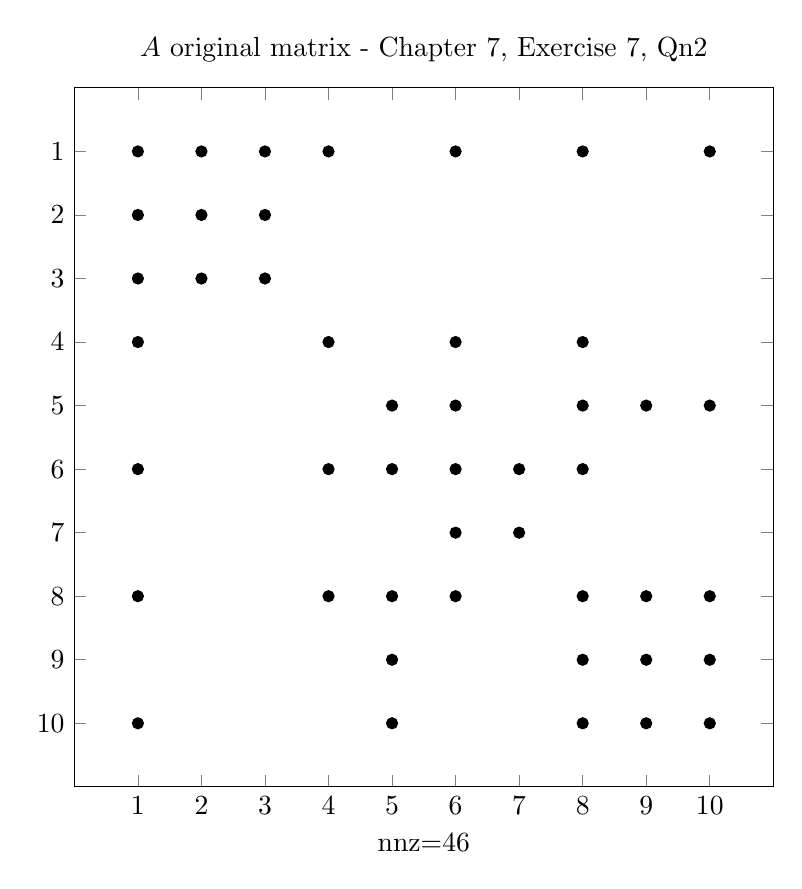
\begin{tikzpicture}
    [   baseline = {(current bounding box.north)}
    ]
    \begin{axis}
        [   unit vector ratio* = 1 1 1
        ,   y dir = reverse
        ,   xmin = 0
        ,   ymin = 0
        ,   xmax = 11
        ,   ymax = 11
        ,   title = {$A$ original matrix - Chapter 7, Exercise 7, Qn2}
        ,   xlabel = {nnz=46}
        ,   width = \linewidth
        ,   xtick = {1,2,3,4,5,6,7,8,9,10}
        ,   ytick = {1,2,3,4,5,6,7,8,9,10}
        ]
        \addplot[only marks] coordinates
        {   (1,1)(2,1)(3,1)(4,1)     (6,1)     (8,1)     (10,1)
            (1,2)(2,2)(3,2)
            (1,3)(2,3)(3,3)
            (1,4)          (4,4)     (6,4)     (8,4)
                                (5,5)(6,5)     (8,5)(9,5)(10,5)
            (1,6)          (4,6)(5,6)(6,6)(7,6)(8,6)
                                     (6,7)(7,7)
            (1,8)          (4,8)(5,8)(6,8)     (8,8)(9,8)(10,8)
                                (5,9)          (8,9)(9,9)(10,9)
            (1,10)              (5,10)      (8,10)(9,10)(10,10)
        };
    \end{axis}
\end{tikzpicture}
\end{center}

    \end{minipage}

    You can find the hald bandwitch of $A$ using the following commands:
    \begin{lstlisting}
>> [i,j]=find(A);
>> bw=max(i-j)

bw =
    9
    \end{lstlisting}
    Therefore the full bandwidth is $= 9 + 9 + 1 = 19$

    Next we apply the Cuthill-McKee (CM) and reverse Cuthill-McKee (RCM)
    ordering algorithms to reduce the bandwidth.

    we need to construct the following table
    \begin{center}
        \renewcommand{\arraystretch}{1.2}
        \setlength{\tabcolsep}{6pt}
        \begin{tabular}{p{15mm}p{20mm}p{15mm}p{18mm}p{16mm}p{16mm}p{15mm}}
            Original nodes & No. of connections & Results / Heads & Queue
            & Result by CM & Result by RCM & New nodes\\
            \hline
             1 & 6 &  7 & 6\\
             2 & 2 &  6 & 4, 5, 8, 1\\
             3 & 2 &  4 & --\\
             4 & 3 &  5 & 9, 10\\
             5 & 4 &  8 & --\\
             6 & 5 &  1 & 2, 3\\
             7 & 1 &  9 & --\\
             8 & 6 & 10 & --\\
             9 & 3 &  2 & --\\
            10 & 4 &  3 & --\\
        \end{tabular}
    \end{center}
    Step 1 - list all the nodes and the number of their connections (or degree)
    -- check this with the adjacency matrix as well.

    Step 2 - choose the node with smallest number of connections --  here is
    node 7 -- write it down under the Results/Heads column.
    Since node 7 is only connected to node 6 we write down 6 Queue column.
    Bring down 6 to the results column,

    Step 3 - next, in the Queue column write down the list of nodes which are
    connected to 6 (in the ascending order of their degree or number of
    connections).
    Bring 4 down and repeat Stage 3.
    Avoid writing the numbers which are already listed in the Queue column and
    the starting node 7 -- since 6, 1, and 8 are already in the Queue we put a
    -- for node 4 in the Queue column.

    Step 4 - we bring the next number down in the queue -- that is 5, and repeat
    stage 3.
    We only list 9 and 10, since 6 and 8 are already listed in the queue.

    Repeat Step 4 -- all the connections to node 8 already in the list, so we
    put a -- for node 8 in the Queue column.

    We bring 1 down which is connected to two new nodes 2 and 3, we write down
    2, 3 in the Queue column.

    Next, we bring 9 and follow the above procedure until all 10 nodes are
    listed in the results/Head column.

    \begin{center}
        \renewcommand{\arraystretch}{1.2}
        \setlength{\tabcolsep}{6pt}
        \begin{tabular}{p{15mm}p{20mm}p{15mm}p{18mm}p{16mm}p{16mm}p{15mm}}
            Original nodes & No. of connections & Results / Heads & Queue
            & Result by CM & Result by RCM & New nodes\\
            \hline
             1 & 6 &  7 & 6 &  7 & \tikzmark{B}3\tikzmark{C} & \tikzmark{D}1\\
             2 & 2 &  6 & 4, 5, 8, 1 &  6 &  2 &  2\\
             3 & 2 &  4 & --         &  4 & 10 &  3\\
             4 & 3 &  5 & 9, 10      &  5 &  9 &  4\\
             5 & 4 &  8 & --         &  8 &  1 &  5\\
             6 & 5 &  1 & 2, 3       &  1 &  8 &  6\\
             7 & 1 &  9 & --         &  9 &  5 &  7\\
             8 & 6 & 10 & --         & 10 &  4 &  8\\
             9 & 3 &  2 & --         &  2 &  6 &  9\\
            10 & 4 &  3 & -- &  3\tikzmark{A} &  7 & 10\\
        \end{tabular}
        \begin{tikzpicture}
            [   remember picture
            ,   overlay
            ,   > = Stealth
            ]
            \draw[<->] ($(pic cs:A)+(4pt,6pt)$) to[out=45, in=-135] ($(pic cs:B)+(-4pt,2pt)$);
            \draw[->] ($(pic cs:C)+(4pt,4pt)$) to ($(pic cs:D)+(-4pt,4pt)$);
        \end{tikzpicture}
    \end{center}

    Complete results column for CM (the same as the column Results / Heads) and
    then reverse the CM column for RCM method, and enter the column header
    `New nodes'.

    We now copy the original adjacency graph and go along the RCM column, and
    say that, the original node 3 becomes node 1, original node 2 remains node 2,
    original node 10 becomes 3, and so on.

    Repeat this for CM method.

    \begin{center}
        \includegraphics[width=0.45\linewidth]{main/07/ch7ex3orig.tikz}

        \vspace{1em}
        \includegraphics[width=0.45\linewidth]{main/07/ch7ex3cm.tikz}
        \hspace{\fill}
        \includegraphics[width=0.45\linewidth]{main/07/ch7ex3rcm.tikz}
    \end{center}

    \newpage
    Now use MATLAB to construct the adjacency matrix B and C associated with the
    reordered RCM adjacency plot:

    \begin{minipage}[t]{0.49\linewidth}
        \vspace{-2em}
        \begin{lstlisting}
B=[
    1 1 0 0 0 0 0 0 0 0
    1 1 1 1 1 1 0 0 0 0
    0 1 1 0 1 1 0 0 0 0
    0 1 0 1 1 0 1 1 0 0
    0 1 1 1 1 1 1 1 0 0
    0 1 1 0 1 1 0 1 1 1
    0 0 0 1 1 0 1 1 0 0
    0 0 0 1 1 1 1 1 0 0
    0 0 0 0 0 1 0 0 1 1
    0 0 0 0 0 1 0 0 1 1];
        \end{lstlisting}

        We can now find the bandwidth for the reordered matrix:
        \begin{lstlisting}
>> [i,j]=find(B);
>> bw=max(i-j)

bw = 4
        \end{lstlisting}
    \end{minipage}
    \begin{minipage}[t]{0.5\linewidth}
        \begin{center}
\scriptsize
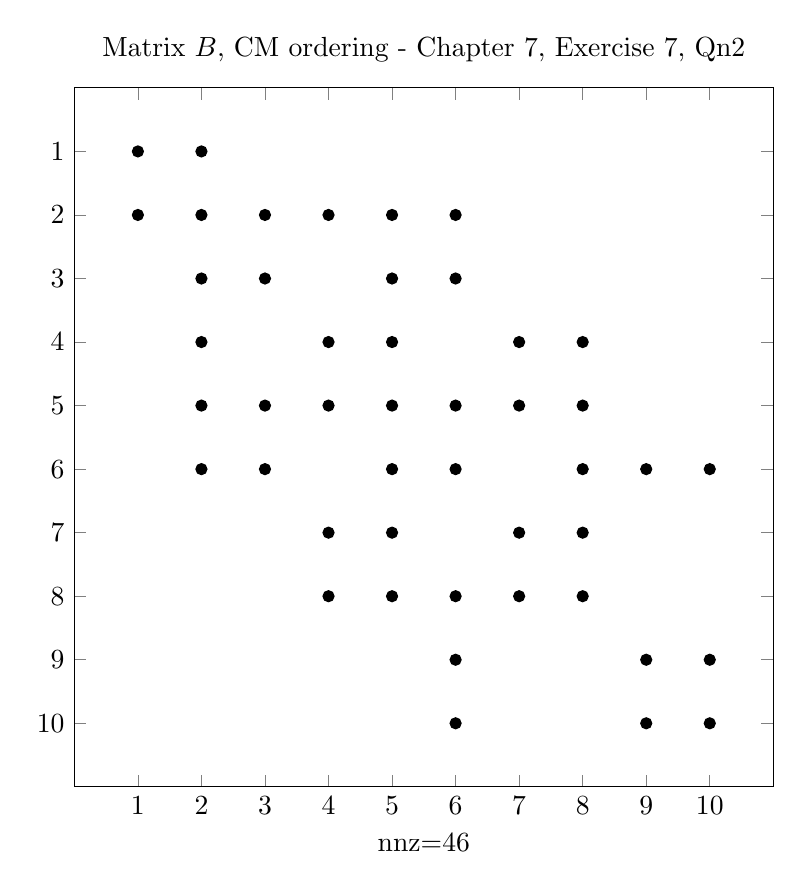
\begin{tikzpicture}
    [   baseline = {(current bounding box.north)}
    ]
    \begin{axis}
        [   unit vector ratio* = 1 1 1
        ,   y dir = reverse
        ,   xmin = 0
        ,   ymin = 0
        ,   xmax = 11
        ,   ymax = 11
        ,   title = {Matrix $B$, CM ordering - Chapter 7, Exercise 7, Qn2}
        ,   xlabel = {nnz=46}
        ,   width = \linewidth
        ,   xtick = {1,2,3,4,5,6,7,8,9,10}
        ,   ytick = {1,2,3,4,5,6,7,8,9,10}
        ]
        \addplot[only marks] coordinates
        {   (1,1)(2,1)
            (1,2)(2,2)(3,2)(4,2)(5,2)(6,2)
                 (2,3)(3,3)     (5,3)(6,3)
                 (2,4)     (4,4)(5,4)     (7,4)(8,4)
                 (2,5)(3,5)(4,5)(5,5)(6,5)(7,5)(8,5)
                 (2,6)(3,6)     (5,6)(6,6)     (8,6)(9,6)(10,6)
                           (4,7)(5,7)     (7,7)(8,7)
                           (4,8)(5,8)(6,8)(7,8)(8,8)
                                     (6,9)          (9,9)(10,9)
                                     (6,10)        (9,10)(10,10)
        };
    \end{axis}
\end{tikzpicture}
\end{center}

    \end{minipage}

    Hence, the full bandwidth for the reordered matrix by CM method is
    $= 4 + 4 + 1 = 9$.

    \begin{minipage}[t]{0.49\linewidth}
        \begin{lstlisting}
C=[
    1 1 0 0 1 0 0 0 0 0
    1 1 0 0 1 0 0 0 0 0
    0 0 1 1 1 1 1 0 0 0
    0 0 1 1 0 1 1 0 0 0
    1 1 1 0 1 1 0 1 1 0
    0 0 1 1 1 1 1 1 1 0
    0 0 1 1 0 1 1 0 1 0
    0 0 0 0 1 1 0 1 1 0
    0 0 0 0 1 1 1 1 1 1
    0 0 0 0 0 0 0 0 1 1];
        \end{lstlisting}

        \begin{lstlisting}
>> [i,j]=find(B);
>> bw=max(i-j)

bw = 4
        \end{lstlisting}
    \end{minipage}
    \begin{minipage}[t]{0.5\linewidth}
        \begin{center}
\scriptsize
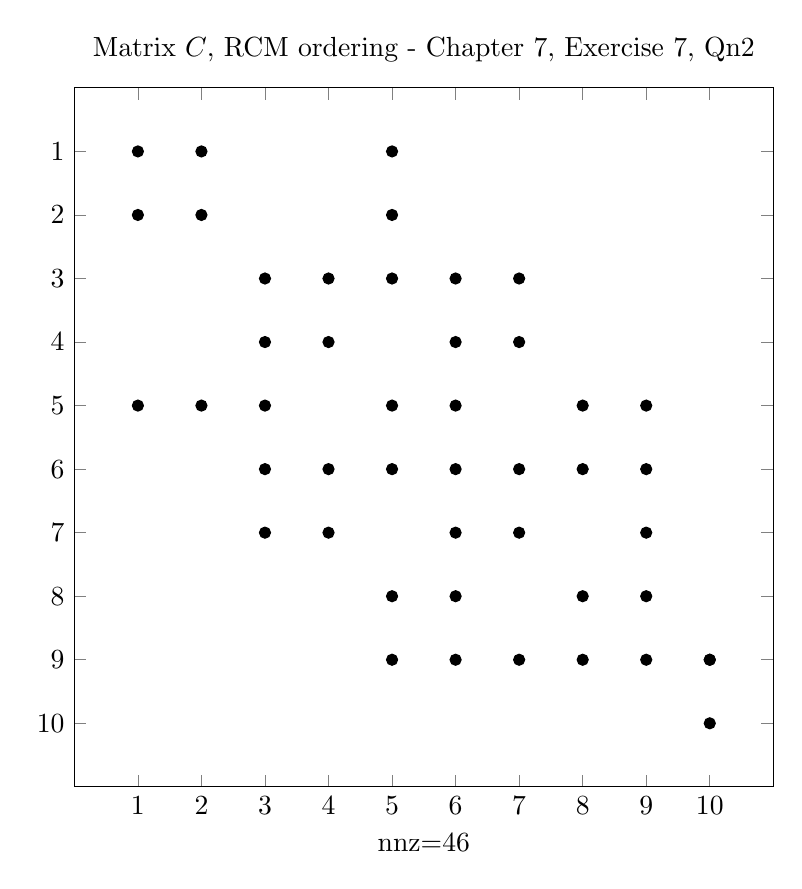
\begin{tikzpicture}
    [   baseline = {(current bounding box.north)}
    ]
    \begin{axis}
        [   unit vector ratio* = 1 1 1
        ,   y dir = reverse
        ,   xmin = 0
        ,   ymin = 0
        ,   xmax = 11
        ,   ymax = 11
        ,   title = {Matrix $C$, RCM ordering - Chapter 7, Exercise 7, Qn2}
        ,   xlabel = {nnz=46}
        ,   width = \linewidth
        ,   xtick = {1,2,3,4,5,6,7,8,9,10}
        ,   ytick = {1,2,3,4,5,6,7,8,9,10}
        ]
        \addplot[only marks] coordinates
        {   (1,1)(2,1)          (5,1)
            (1,2)(2,2)          (5,2)
                      (3,3)(4,3)(5,3)(6,3)(7,3)
                      (3,4)(4,4)     (6,4)(7,4)
            (1,5)(2,5)(3,5)     (5,5)(6,5)     (8,5)(9,5)
                      (3,6)(4,6)(5,6)(6,6)(7,6)(8,6)(9,6)
                      (3,7)(4,7)     (6,7)(7,7)     (9,7)
                                (5,8)(6,8)     (8,8)(9,8)
                                (5,9)(6,9)(7,9)(8,9)(9,9)(10,9)
                                                   (10,9)(10,10)
        };
    \end{axis}
\end{tikzpicture}
\end{center}

    \end{minipage}

    Hence, the full bandwidth for the reordered matrix by CM method is
    $= 4 + 4 + 1 = 9$.

    For this example matrix, both CM and RCM work equally well in reducing the
    bandwidth of the original matrix from 19 to 9.

    \newpage
    Next we use the MATLAB command \texttt{symrcm(A)} to test our RCM reordering
    result.

    \begin{minipage}[t]{0.49\linewidth}
        \begin{lstlisting}
>> p=symrcm(A);
>> spy(A(p,p))
        \end{lstlisting}

        Next we can find the corresponding bandwidth:

        \begin{lstlisting}
>> [i,j]=find(A(p,p));
>> bw=max(i-j)

bw = 4
        \end{lstlisting}

        Hence, the \texttt{symrcm} command also results in a full bandwidth of
        $= 4 + 4 + 1 = 9$.
    \end{minipage}
    \begin{minipage}[t]{0.5\linewidth}
        \begin{center}
\scriptsize
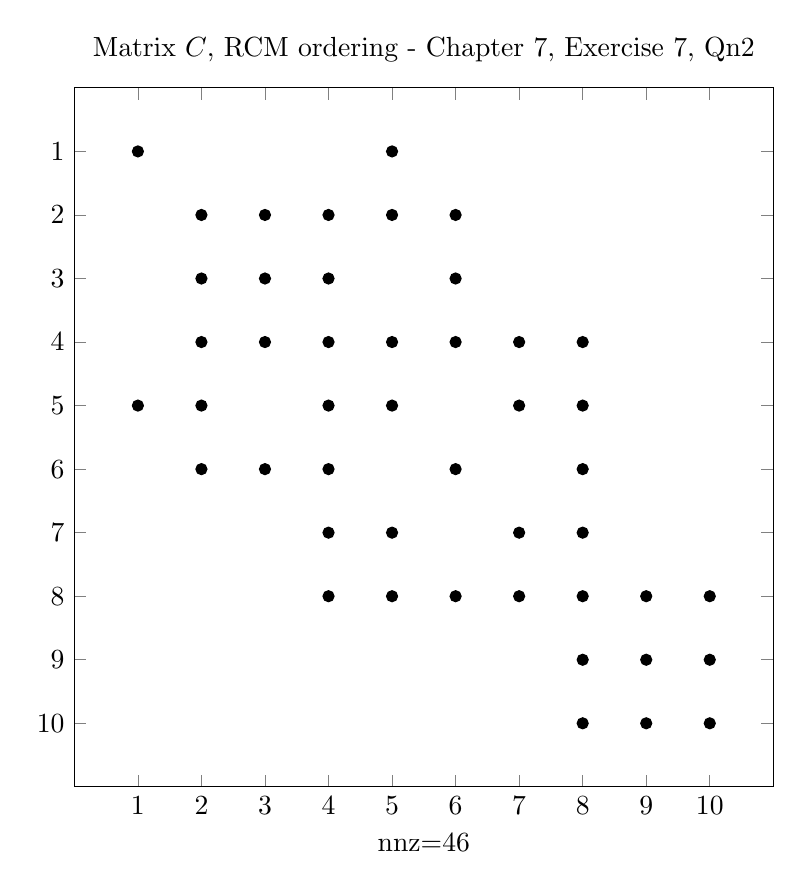
\begin{tikzpicture}
    [   baseline = {(current bounding box.north)}
    ]
    \begin{axis}
        [   unit vector ratio* = 1 1 1
        ,   y dir = reverse
        ,   xmin = 0
        ,   ymin = 0
        ,   xmax = 11
        ,   ymax = 11
        ,   title = {Matrix $C$, RCM ordering - Chapter 7, Exercise 7, Qn2}
        ,   xlabel = {nnz=46}
        ,   width = \linewidth
        ,   xtick = {1,2,3,4,5,6,7,8,9,10}
        ,   ytick = {1,2,3,4,5,6,7,8,9,10}
        ]
        \addplot[only marks] coordinates
        {   (1,1)               (5,1)
                 (2,2)(3,2)(4,2)(5,2)(6,2)
                 (2,3)(3,3)(4,3)     (6,3)
                 (2,4)(3,4)(4,4)(5,4)(6,4)(7,4)(8,4)
            (1,5)(2,5)     (4,5)(5,5)     (7,5)(8,5)
                 (2,6)(3,6)(4,6)     (6,6)     (8,6)
                           (4,7)(5,7)     (7,7)(8,7)
                           (4,8)(5,8)(6,8)(7,8)(8,8)(9,8)(10,8)
                                               (8,9)(9,9)(10,9)
                                              (8,10)(9,10)(10,10)
        };
    \end{axis}
\end{tikzpicture}
\end{center}

    \end{minipage}

    Reading form the plot of \texttt{symrcm} adjacency matrix, we can also write
    down the associated adjacency matrix and plot:

    \begin{minipage}[t]{0.49\linewidth}
        \begin{lstlisting}
A(p,p)=[
    1 0 0 0 1 0 0 0 0 0
    0 1 1 1 1 1 0 0 0 0
    0 1 1 1 0 1 0 0 0 0
    0 1 1 1 1 1 1 1 0 0
    1 1 0 1 1 0 1 1 0 0
    0 1 1 1 0 1 0 1 0 0
    0 0 0 1 1 1 1 1 1 1
    0 0 0 0 0 0 0 1 1 1
    0 0 0 0 0 0 0 1 1 1]
        \end{lstlisting}
    \end{minipage}
    \begin{minipage}[t]{0.5\linewidth}
        ~\\
        \includegraphics[width=0.9\linewidth]{main/07/ch7ex3sym.tikz}
    \end{minipage}

    \newpage
    \textbf{Column Count reordering:}

    \begin{center}
        \renewcommand{\arraystretch}{1.2}
        \setlength{\tabcolsep}{6pt}
        \begin{tabular}{r|>{\hspace*{\tabcolsep}}CCCCCCCCCC}
            vertex & 1 & 2 & 3 & 4 & 5 & 6 & 7 & 8 & 9 & 10\\
            \hline
            degree & 6 & 2 & 2 & 3 & 4 & 5 & 1 & 6 & 3 & 4\\
        \end{tabular}

        \begin{tabular}{r|>{\hspace*{\tabcolsep}}CCCCCCCCCC}
            vertex   & 1 & 2 & 3 & 4 & 5 & 6 & 7 & 8 & 9 & 10\\
            \hline
            original & 7\uparrow & 2\uparrow & 3\uparrow & 4\uparrow & 9\uparrow & 5\uparrow &10\uparrow & 6\uparrow & 1\uparrow & 8\uparrow\\
        \end{tabular}
    \end{center}
    \vspace{2em}
    \begin{center}
        \renewcommand{\arraystretch}{1.2}
        \setlength{\tabcolsep}{2ex}
        \begin{tabular}{p{0.45\linewidth}|p{0.45\linewidth}}
            \centering\includegraphics[width=0.9\linewidth]{main/07/ch7ex3orig.tikz} &
            \centering\includegraphics[width=0.9\linewidth]{main/07/ch7ex3cc.tikz}
            \arraybackslash\\
            ~\vspace{2em}

            $\scriptsize D = \begin{pmatrix}
                1 & 0 & 0 & 0 & 0 & 0 & 0 & 1 & 0 & 0\\
                0 & 1 & 1 & 0 & 0 & 0 & 0 & 0 & 1 & 0\\
                0 & 1 & 1 & 0 & 0 & 0 & 0 & 0 & 1 & 0\\
                0 & 0 & 0 & 1 & 0 & 0 & 0 & 1 & 1 & 1\\
                0 & 0 & 0 & 0 & 1 & 1 & 1 & 0 & 0 & 1\\
                0 & 0 & 0 & 0 & 1 & 1 & 1 & 1 & 0 & 1\\
                0 & 0 & 0 & 0 & 1 & 1 & 1 & 0 & 1 & 1\\
                1 & 0 & 0 & 1 & 0 & 1 & 0 & 1 & 1 & 1\\
                0 & 1 & 1 & 1 & 0 & 0 & 1 & 1 & 1 & 1\\
                0 & 0 & 0 & 1 & 1 & 1 & 1 & 1 & 1 & 1
            \end{pmatrix}$ &
            \begin{center}
\scriptsize
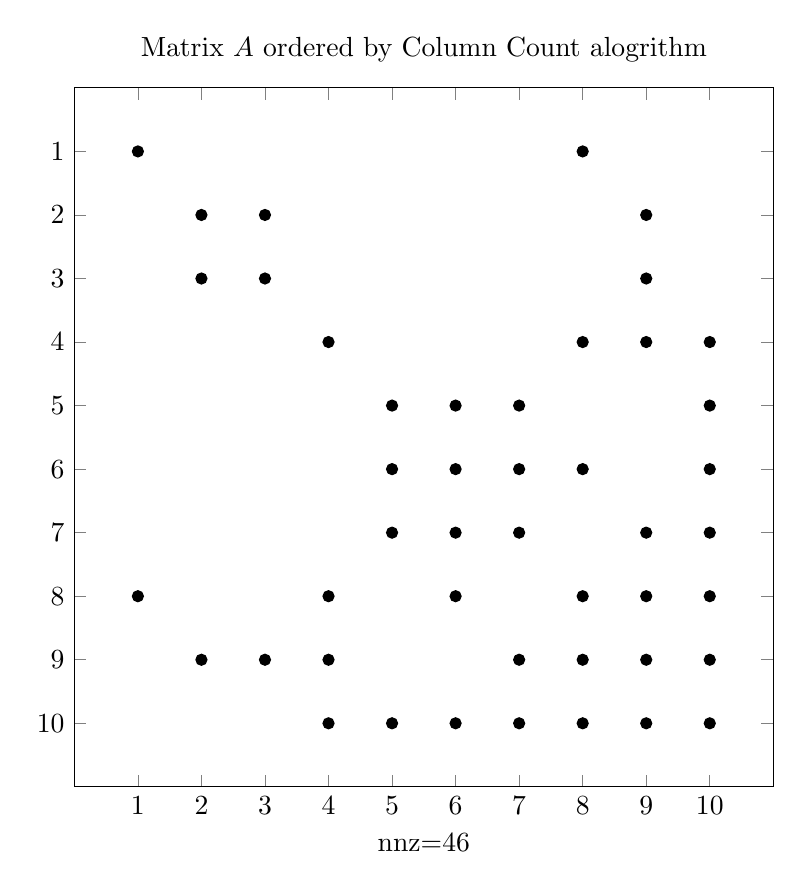
\begin{tikzpicture}
    [   baseline = {(current bounding box.north)}
    ]
    \begin{axis}
        [   unit vector ratio* = 1 1 1
        ,   y dir = reverse
        ,   xmin = 0
        ,   ymin = 0
        ,   xmax = 11
        ,   ymax = 11
        ,   title = {Matrix $A$ ordered by Column Count alogrithm}
        ,   xlabel = {nnz=46}
        ,   width = \linewidth
        ,   xtick = {1,2,3,4,5,6,7,8,9,10}
        ,   ytick = {1,2,3,4,5,6,7,8,9,10}
        ]
        \addplot[only marks] coordinates
        {   (1,1)                              (8,1)
                 (2,2)(3,2)                         (9,2)
                 (2,3)(3,3)                         (9,3)
                           (4,4)               (8,4)(9,4)(10,4)
                                (5,5)(6,5)(7,5)          (10,5)
                                (5,6)(6,6)(7,6)(8,6)     (10,6)
                                (5,7)(6,7)(7,7)     (9,7)(10,7)
            (1,8)          (4,8)     (6,8)     (8,8)(9,8)(10,8)
                 (2,9)(3,9)(4,9)          (7,9)(8,9)(9,9)(10,9)
                    (4,10)(5,10)(6,10)(7,10)(8,10)(9,10)(10,10)
        };
    \end{axis}
\end{tikzpicture}
\end{center}

            \\
            ~\vspace{2em}

            Note that D (ordered Matrix $A$ by Column Count algorithm) is identical to Matrix A ordered by using the MATLAB command \texttt{colperm} i.e.

            \begin{lstlisting}
>> q=colperm(A);
>> spy(A(q,q))
            \end{lstlisting}&
            \begin{center}
\scriptsize
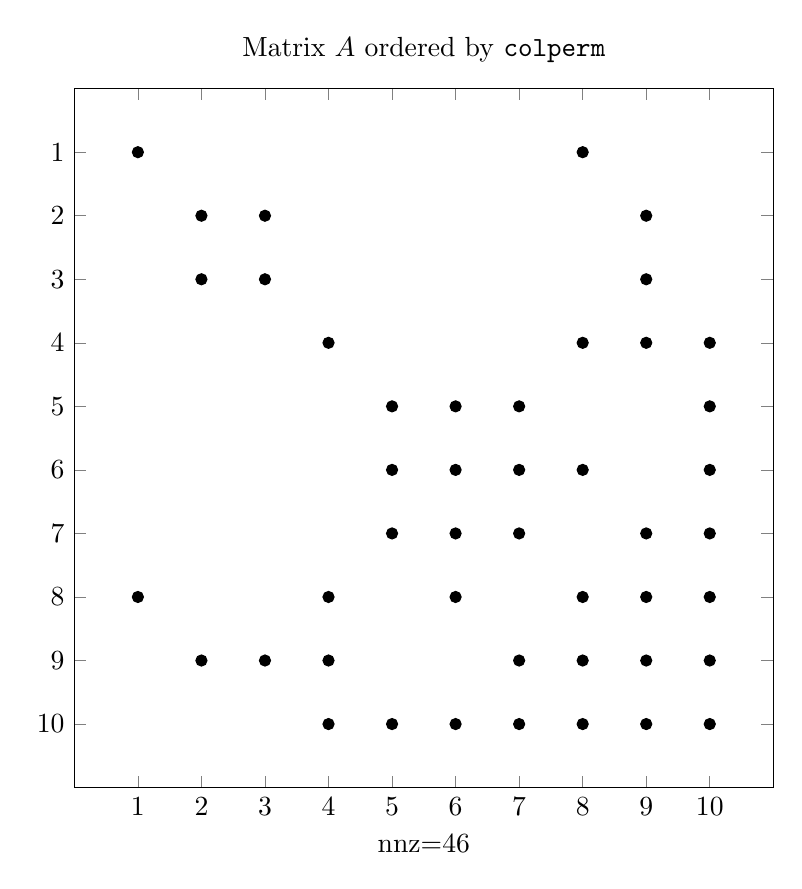
\begin{tikzpicture}
    [   baseline = {(current bounding box.north)}
    ]
    \begin{axis}
        [   unit vector ratio* = 1 1 1
        ,   y dir = reverse
        ,   xmin = 0
        ,   ymin = 0
        ,   xmax = 11
        ,   ymax = 11
        ,   title = {Matrix $A$ ordered by \texttt{colperm}}
        ,   xlabel = {nnz=46}
        ,   width = \linewidth
        ,   xtick = {1,2,3,4,5,6,7,8,9,10}
        ,   ytick = {1,2,3,4,5,6,7,8,9,10}
        ]
        \addplot[only marks] coordinates
        {   (1,1)                              (8,1)
                 (2,2)(3,2)                         (9,2)
                 (2,3)(3,3)                         (9,3)
                           (4,4)               (8,4)(9,4)(10,4)
                                (5,5)(6,5)(7,5)          (10,5)
                                (5,6)(6,6)(7,6)(8,6)     (10,6)
                                (5,7)(6,7)(7,7)     (9,7)(10,7)
            (1,8)          (4,8)     (6,8)     (8,8)(9,8)(10,8)
                 (2,9)(3,9)(4,9)          (7,9)(8,9)(9,9)(10,9)
                    (4,10)(5,10)(6,10)(7,10)(8,10)(9,10)(10,10)
        };
    \end{axis}
\end{tikzpicture}
\end{center}

        \end{tabular}
    \end{center}

    \newpage
    \textbf{Minimum Degree reordering}

    \begin{center}
        \renewcommand{\arraystretch}{1}
        \setlength{\tabcolsep}{8pt}
        \begin{tabular}{rr|cccccccccc}
            \multicolumn{2}{l|}{New} & \multicolumn{10}{c}{vertex and number of degree}\\
            \multicolumn{2}{l|}{ordering} & 1 & 2 & 3 & 4 & 5 & 6 & 7 & 8 & 9 & 10\\
            \multicolumn{2}{C|}{\leftarrow} & 6 & 2 & 2 & 3 & 4 & 5 & 1 & 6 & 3 & 4\\
            \hline
            1 & 7 & 6 & 2 & 2 & 3 & 4 & 4 & X & 6 & 3 & 4\\
            2 & 2 & 5 & X & 1 & 3 & 4 & 4 & X & 6 & 3 & 4\\
            3 & 3 & 4 & X & X & 3 & 4 & 4 & X & 5 & 3 & 4\\
            4 & 4 & 3 & X & X & X & 4 & 3 & X & 5 & 3 & 4\\
            5 & 1 & X & X & X & X & 4 & 2 & X & 4 & 3 & 3\\
            6 & 6 & X & X & X & X & 3 & X & X & 3 & 3 & 3\\
            7 & 8 & X & X & X & X & 2 & X & X & X & 2 & 2\\
            8 & 5 & X & X & X & X & X & X & X & X & 1 & 1\\
            9 & 9 & X & X & X & X & X & X & X & X & X & 1\\
            10&10 & X & X & X & X & X & X & X & X & X & X\\
        \end{tabular}
    \end{center}
    \begin{center}
        \renewcommand{\arraystretch}{1}
        \setlength{\tabcolsep}{6pt}
        \begin{tabular}{p{0.45\linewidth}|p{0.45\linewidth}}
            ~\vspace{2em}

            $\scriptsize M = \begin{pmatrix}
                1 & 0 & 0 & 0 & 0 & 1 & 0 & 0 & 0 & 0\\
                0 & 1 & 1 & 0 & 1 & 0 & 0 & 0 & 0 & 0\\
                0 & 1 & 1 & 0 & 1 & 0 & 0 & 0 & 0 & 0\\
                0 & 0 & 0 & 1 & 1 & 1 & 1 & 0 & 0 & 0\\
                0 & 1 & 1 & 1 & 1 & 1 & 1 & 0 & 0 & 1\\
                1 & 0 & 0 & 1 & 1 & 1 & 1 & 1 & 0 & 0\\
                0 & 0 & 0 & 1 & 1 & 1 & 1 & 1 & 1 & 1\\
                0 & 0 & 0 & 0 & 0 & 0 & 1 & 1 & 1 & 1\\
                0 & 0 & 0 & 0 & 1 & 0 & 1 & 1 & 1 & 1
            \end{pmatrix}$ &
            ~\vspace{-2em}

            \centering\includegraphics[width=0.9\linewidth]{main/07/ch7ex3md.tikz}
            \arraybackslash\\
            \begin{center}
\scriptsize
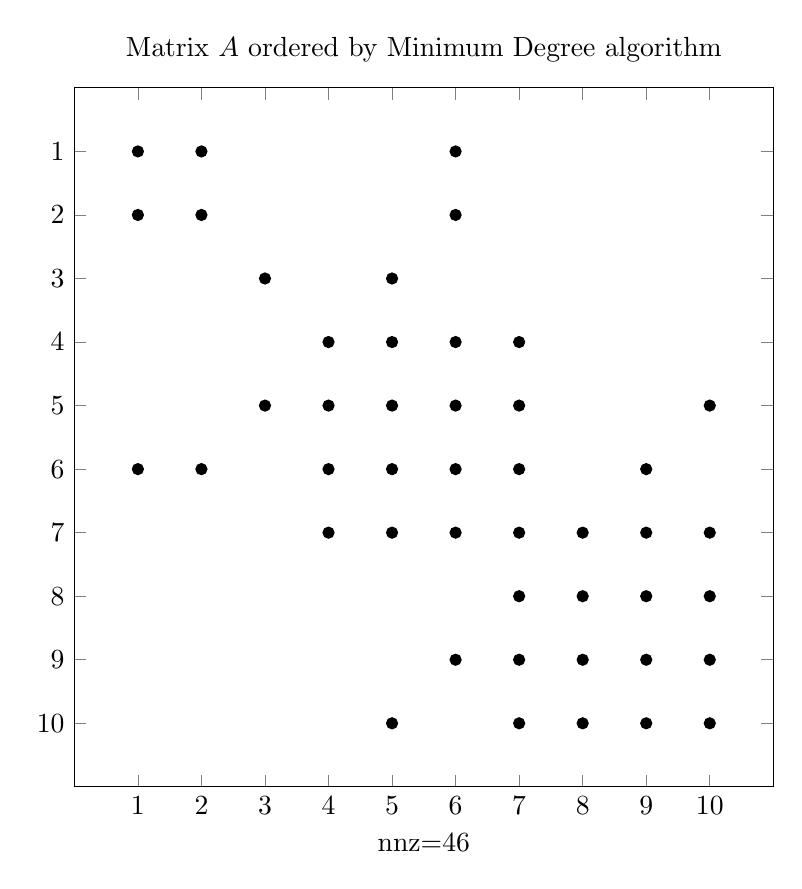
\begin{tikzpicture}
    [   baseline = {(current bounding box.north)}
    ]
    \begin{axis}
        [   unit vector ratio* = 1 1 1
        ,   y dir = reverse
        ,   xmin = 0
        ,   ymin = 0
        ,   xmax = 11
        ,   ymax = 11
        ,   title = {Matrix $A$ ordered by Minimum Degree algorithm}
        ,   xlabel = {nnz=46}
        ,   width = \linewidth
        ,   xtick = {1,2,3,4,5,6,7,8,9,10}
        ,   ytick = {1,2,3,4,5,6,7,8,9,10}
        ]
        \addplot[only marks] coordinates
        {   (1,1)(2,1)               (6,1)
            (1,2)(2,2)               (6,2)
                      (3,3)     (5,3)
                           (4,4)(5,4)(6,4)(7,4)
                      (3,5)(4,5)(5,5)(6,5)(7,5)          (10,5)
            (1,6)(2,6)     (4,6)(5,6)(6,6)(7,6)     (9,6)
                           (4,7)(5,7)(6,7)(7,7)(8,7)(9,7)(10,7)
                                          (7,8)(8,8)(9,8)(10,8)
                                     (6,9)(7,9)(8,9)(9,9)(10,9)
                                (5,10)  (7,10)(8,10)(9,10)(10,10)
        };
    \end{axis}
\end{tikzpicture}
\end{center}
 &
            \begin{center}
\scriptsize
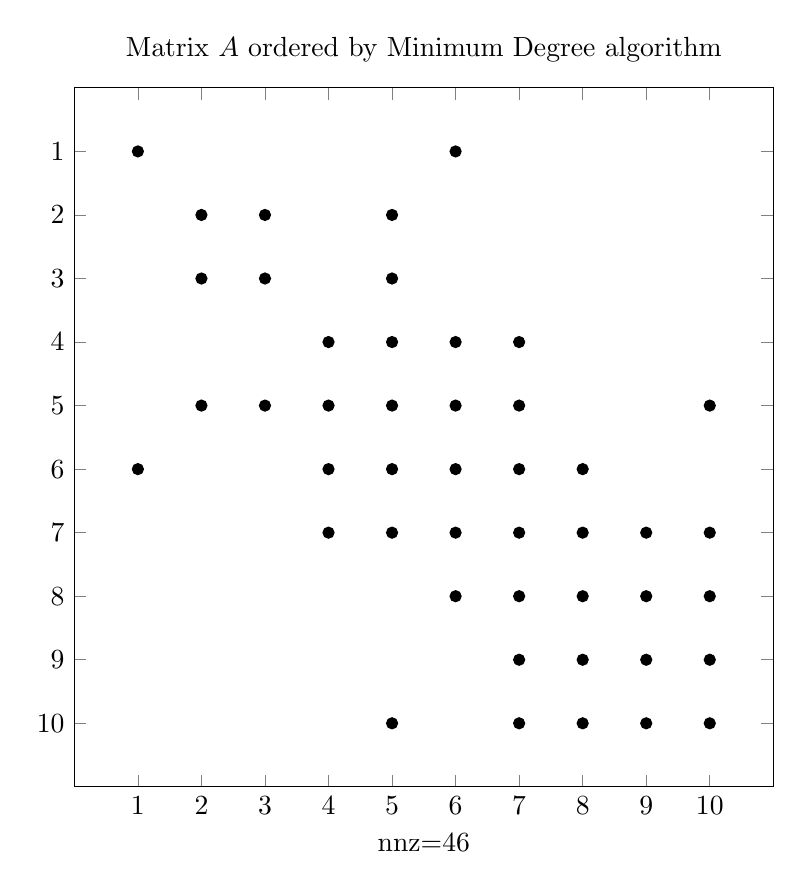
\begin{tikzpicture}
    [   baseline = {(current bounding box.north)}
    ]
    \begin{axis}
        [   unit vector ratio* = 1 1 1
        ,   y dir = reverse
        ,   xmin = 0
        ,   ymin = 0
        ,   xmax = 11
        ,   ymax = 11
        ,   title = {Matrix $A$ ordered by Minimum Degree algorithm}
        ,   xlabel = {nnz=46}
        ,   width = \linewidth
        ,   xtick = {1,2,3,4,5,6,7,8,9,10}
        ,   ytick = {1,2,3,4,5,6,7,8,9,10}
        ]
        \addplot[only marks] coordinates
        {   (1,1)                    (6,1)
                 (2,2)(3,2)     (5,2)
                 (2,3)(3,3)     (5,3)
                           (4,4)(5,4)(6,4)(7,4)
                 (2,5)(3,5)(4,5)(5,5)(6,5)(7,5)          (10,5)
            (1,6)          (4,6)(5,6)(6,6)(7,6)(8,6)
                           (4,7)(5,7)(6,7)(7,7)(8,7)(9,7)(10,7)
                                     (6,8)(7,8)(8,8)(9,8)(10,8)
                                          (7,9)(8,9)(9,9)(10,9)
                                (5,10)  (7,10)(8,10)(9,10)(10,10)
        };
    \end{axis}
\end{tikzpicture}
\end{center}
\\
        \end{tabular}
    \end{center}

    \textbf{Comment} -- for this matrix, the MD algorithm seems to produce a
    reordered matrix very similar to the \texttt{sysamd} function within MATLAB,
    hence the algorithm works well.

    \textbf{Next we perform LU factorisation and check the number of nonzeros
    generated in the decomposition process}.

    See Figure 7.Q2, below. Compare the upper triangular matrix $U$ in each case
    with the corresponding full matrices, i.e. original matrix $A$, RCM ($C$),
    Column Count ($D$) and Minimum Degree ($M$), and write down the number of
    nonzeros generated for each case.
    The answer will be checked in the tutorial session.

    \begin{center}
        \renewcommand{\arraystretch}{0.6}
        \setlength{\tabcolsep}{6pt}
        \begin{tabular}{p{0.45\linewidth} p{0.45\linewidth}}
            \begin{center}
\scriptsize
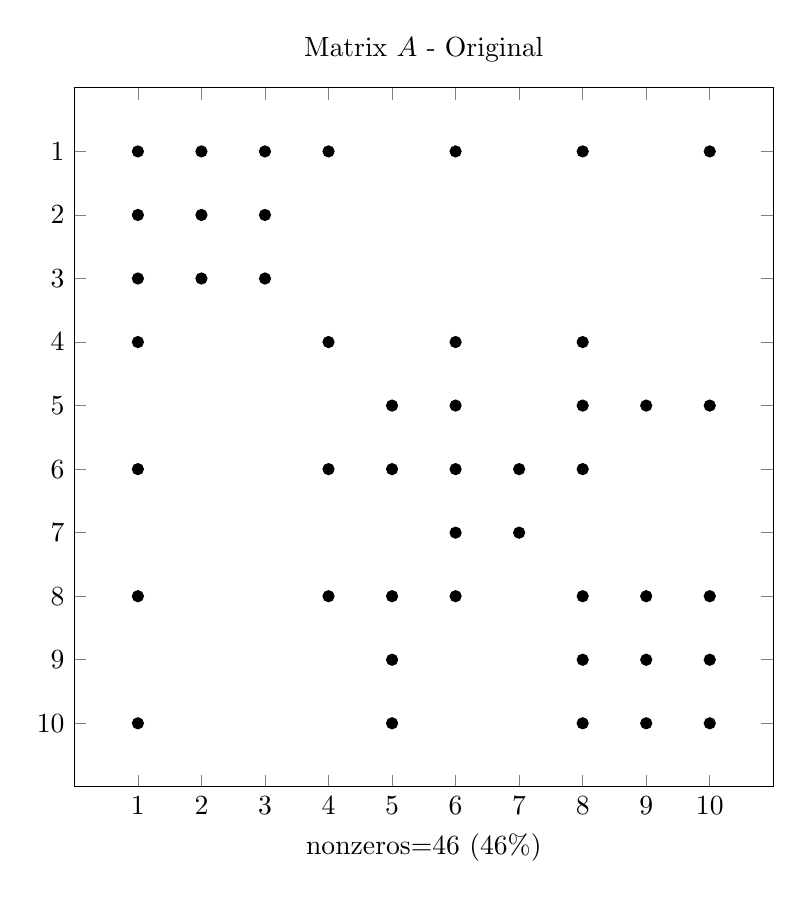
\begin{tikzpicture}
    [   baseline = {(current bounding box.north)}
    ]
    \begin{axis}
        [   unit vector ratio* = 1 1 1
        ,   y dir = reverse
        ,   xmin = 0
        ,   ymin = 0
        ,   xmax = 11
        ,   ymax = 11
        ,   title = {Matrix $A$ - Original}
        ,   xlabel = {nonzeros=46 (46\%)}
        ,   width = \linewidth
        ,   xtick = {1,2,3,4,5,6,7,8,9,10}
        ,   ytick = {1,2,3,4,5,6,7,8,9,10}
        ]
        \addplot[only marks] coordinates
        {   (1,1)(2,1)(3,1)(4,1)     (6,1)     (8,1)     (10,1)
            (1,2)(2,2)(3,2)
            (1,3)(2,3)(3,3)
            (1,4)          (4,4)     (6,4)     (8,4)
                                (5,5)(6,5)     (8,5)(9,5)(10,5)
            (1,6)          (4,6)(5,6)(6,6)(7,6)(8,6)
                                     (6,7)(7,7)
            (1,8)          (4,8)(5,8)(6,8)     (8,8)(9,8)(10,8)
                                (5,9)          (8,9)(9,9)(10,9)
            (1,10)              (5,10)      (8,10)(9,10)(10,10)
        };
    \end{axis}
\end{tikzpicture}
\end{center}
 & \begin{center}
\scriptsize
\begin{tikzpicture}
    [   baseline = {(current bounding box.north)}
    ]
    \begin{axis}
        [   unit vector ratio* = 1 1 1
        ,   y dir = reverse
        ,   xmin = 0
        ,   ymin = 0
        ,   xmax = 11
        ,   ymax = 11
        ,   title = {$[L,U]$ of Matrix $A$, $U$}
        ,   xlabel = {nonzeros=38 (38\%)}
        ,   width = \linewidth
        ,   xtick = {1,2,3,4,5,6,7,8,9,10}
        ,   ytick = {1,2,3,4,5,6,7,8,9,10}
        ]
        \addplot[only marks] coordinates
        {   (1,1)(2,1)(3,1)(4,1)     (6,1)     (8,1)     (10,1)
                 (2,2)(3,2)                              (10,2)
                           (4,3)     (6,3)     (8,3)     (10,3)
                           (4,4)     (6,4)     (8,4)     (10,4)
                                (5,5)(6,5)     (8,5)(9,5)(10,5)
                                     (6,6)(7,6)(8,6)(9,6)(10,6)
                                          (7,7)(8,7)(9,7)(10,7)
                                               (8,8)(9,8)(10,8)
                                                    (9,9)(10,9)
                                                         (10,10)
        };
    \end{axis}
\end{tikzpicture}
\end{center}
\\
            \begin{center}
\scriptsize
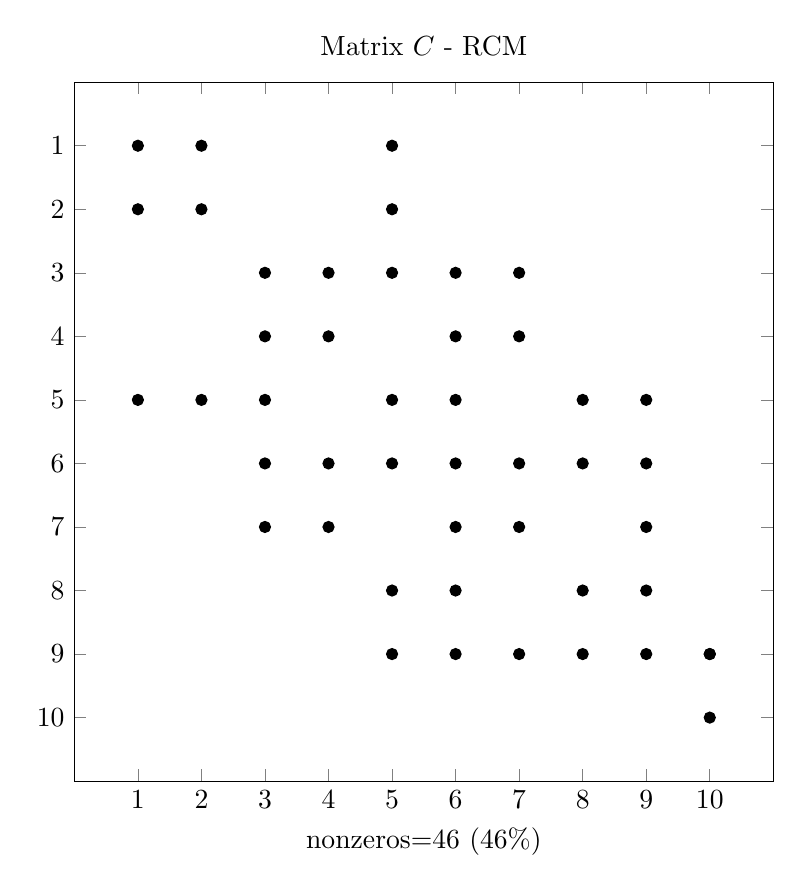
\begin{tikzpicture}
    [   baseline = {(current bounding box.north)}
    ]
    \begin{axis}
        [   unit vector ratio* = 1 1 1
        ,   y dir = reverse
        ,   xmin = 0
        ,   ymin = 0
        ,   xmax = 11
        ,   ymax = 11
        ,   title = {Matrix $C$ - RCM}
        ,   xlabel = {nonzeros=46 (46\%)}
        ,   width = \linewidth
        ,   xtick = {1,2,3,4,5,6,7,8,9,10}
        ,   ytick = {1,2,3,4,5,6,7,8,9,10}
        ]
        \addplot[only marks] coordinates
        {   (1,1)(2,1)          (5,1)
            (1,2)(2,2)          (5,2)
                      (3,3)(4,3)(5,3)(6,3)(7,3)
                      (3,4)(4,4)     (6,4)(7,4)
            (1,5)(2,5)(3,5)     (5,5)(6,5)     (8,5)(9,5)
                      (3,6)(4,6)(5,6)(6,6)(7,6)(8,6)(9,6)
                      (3,7)(4,7)     (6,7)(7,7)     (9,7)
                                (5,8)(6,8)     (8,8)(9,8)
                                (5,9)(6,9)(7,9)(8,9)(9,9)(10,9)
                                                   (10,9)(10,10)
        };
    \end{axis}
\end{tikzpicture}
\end{center}
 & \begin{center}
\scriptsize
\begin{tikzpicture}
    [   baseline = {(current bounding box.north)}
    ]
    \begin{axis}
        [   unit vector ratio* = 1 1 1
        ,   y dir = reverse
        ,   xmin = 0
        ,   ymin = 0
        ,   xmax = 11
        ,   ymax = 11
        ,   title = {$[L,U]$ Matrix $C$, $U$}
        ,   xlabel = {nonzeros=23 (23\%)}
        ,   width = \linewidth
        ,   xtick = {1,2,3,4,5,6,7,8,9,10}
        ,   ytick = {1,2,3,4,5,6,7,8,9,10}
        ]
        \addplot[only marks] coordinates
        {   (1,1)(2,1)          (5,1)

                      (3,3)(4,3)(5,3)(6,3)(7,3)
                           (4,4)(5,4)     (7,4)(8,4)(9,4)
                                (5,5)
                                     (6,6)     (8,6)(9,6)
                                          (7,7)          (10,7)
                                               (8,8)(9,8)
                                                    (9,9)
                                                         (10,10)
        };
    \end{axis}
\end{tikzpicture}
\end{center}
\\
            \begin{center}
\scriptsize
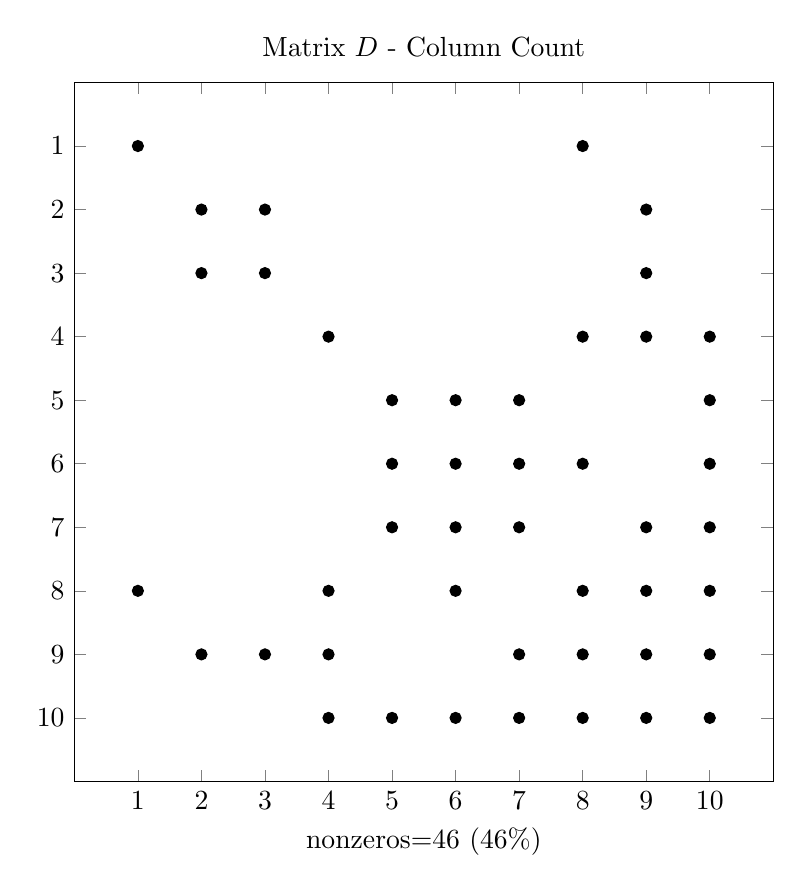
\begin{tikzpicture}
    [   baseline = {(current bounding box.north)}
    ]
    \begin{axis}
        [   unit vector ratio* = 1 1 1
        ,   y dir = reverse
        ,   xmin = 0
        ,   ymin = 0
        ,   xmax = 11
        ,   ymax = 11
        ,   title = {Matrix $D$ - Column Count}
        ,   xlabel = {nonzeros=46 (46\%)}
        ,   width = \linewidth
        ,   xtick = {1,2,3,4,5,6,7,8,9,10}
        ,   ytick = {1,2,3,4,5,6,7,8,9,10}
        ]
        \addplot[only marks] coordinates
        {   (1,1)                              (8,1)
                 (2,2)(3,2)                         (9,2)
                 (2,3)(3,3)                         (9,3)
                           (4,4)               (8,4)(9,4)(10,4)
                                (5,5)(6,5)(7,5)          (10,5)
                                (5,6)(6,6)(7,6)(8,6)     (10,6)
                                (5,7)(6,7)(7,7)     (9,7)(10,7)
            (1,8)          (4,8)     (6,8)     (8,8)(9,8)(10,8)
                 (2,9)(3,9)(4,9)          (7,9)(8,9)(9,9)(10,9)
                    (4,10)(5,10)(6,10)(7,10)(8,10)(9,10)(10,10)
        };
    \end{axis}
\end{tikzpicture}
\end{center}
 & \begin{center}
\scriptsize
\begin{tikzpicture}
    [   baseline = {(current bounding box.north)}
    ]
    \begin{axis}
        [   unit vector ratio* = 1 1 1
        ,   y dir = reverse
        ,   xmin = 0
        ,   ymin = 0
        ,   xmax = 11
        ,   ymax = 11
        ,   title = {$[L,U]$ of Matrix $D$, $U$}
        ,   xlabel = {nonzeros=20 (20\%)}
        ,   width = \linewidth
        ,   xtick = {1,2,3,4,5,6,7,8,9,10}
        ,   ytick = {1,2,3,4,5,6,7,8,9,10}
        ]
        \addplot[only marks] coordinates
        {   (1,1)                              (8,1)
                 (2,2)(3,2)                         (9,2)

                           (4,4)               (8,4)(9,4)(10,4)
                                (5,5)(6,5)(7,5)          (10,5)
                                     (6,6)     (8,6)
                                          (7,7)     (9,7)
                                               (8,8)
                                                    (9,9)
                                                         (10,10)
        };
    \end{axis}
\end{tikzpicture}
\end{center}
\\
            \begin{center}
\scriptsize
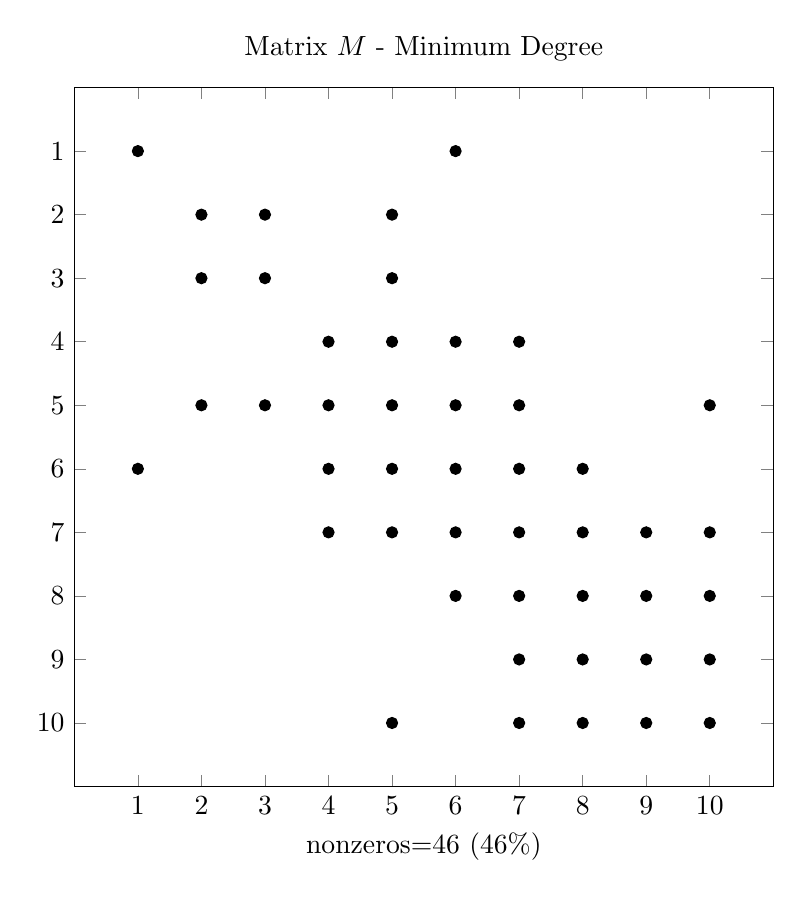
\begin{tikzpicture}
    [   baseline = {(current bounding box.north)}
    ]
    \begin{axis}
        [   unit vector ratio* = 1 1 1
        ,   y dir = reverse
        ,   xmin = 0
        ,   ymin = 0
        ,   xmax = 11
        ,   ymax = 11
        ,   title = {Matrix $M$ - Minimum Degree}
        ,   xlabel = {nonzeros=46 (46\%)}
        ,   width = \linewidth
        ,   xtick = {1,2,3,4,5,6,7,8,9,10}
        ,   ytick = {1,2,3,4,5,6,7,8,9,10}
        ]
        \addplot[only marks] coordinates
        {   (1,1)                    (6,1)
                 (2,2)(3,2)     (5,2)
                 (2,3)(3,3)     (5,3)
                           (4,4)(5,4)(6,4)(7,4)
                 (2,5)(3,5)(4,5)(5,5)(6,5)(7,5)          (10,5)
            (1,6)          (4,6)(5,6)(6,6)(7,6)(8,6)
                           (4,7)(5,7)(6,7)(7,7)(8,7)(9,7)(10,7)
                                     (6,8)(7,8)(8,8)(9,8)(10,8)
                                          (7,9)(8,9)(9,9)(10,9)
                                (5,10)  (7,10)(8,10)(9,10)(10,10)
        };
    \end{axis}
\end{tikzpicture}
\end{center}
 & \begin{center}
\scriptsize
\begin{tikzpicture}
    [   baseline = {(current bounding box.north)}
    ]
    \begin{axis}
        [   unit vector ratio* = 1 1 1
        ,   y dir = reverse
        ,   xmin = 0
        ,   ymin = 0
        ,   xmax = 11
        ,   ymax = 11
        ,   title = {$[L,U]$ Matrix $M$, $U$}
        ,   xlabel = {nonzeros=23 (23\%)}
        ,   width = \linewidth
        ,   xtick = {1,2,3,4,5,6,7,8,9,10}
        ,   ytick = {1,2,3,4,5,6,7,8,9,10}
        ]
        \addplot[only marks] coordinates
        {   (1,1)                    (6,1)
                 (2,2)(3,2)     (5,2)

                           (4,4)(5,4)(6,4)(7,4)
                                (5,5)                    (10,5)
                                     (6,6)     (8,6)
                                          (7,7)(8,7)(9,7)(10,7)
                                               (8,8)(9,8)(10,8)
                                                    (9,9)(10,9)
                                                         (10,10)
        };
    \end{axis}
\end{tikzpicture}
\end{center}
\\
        \end{tabular}
    \end{center}
    Figure 7.Q2 Comparison of ordering schemes (using the algorithms shown in
    \break Chapter 7), and their $LU$ factorisation showing fill-ins reduction.

    \newpage
    \begin{minipage}[t]{0.5\linewidth}
        \begin{align*}
            \scriptsize
            A = \begin{pmatrix}
                1 & 0 & 1 & 0 & 0 & 0 & 0 & 1 & 1\\
                0 & 1 & 1 & 0 & 0 & 0 & 1 & 1 & 0\\
                1 & 1 & 1 & 0 & 0 & 0 & 0 & 0 & 0\\
                0 & 0 & 0 & 1 & 0 & 0 & 0 & 1 & 1\\
                0 & 0 & 0 & 0 & 1 & 0 & 1 & 1 & 0\\
                0 & 0 & 0 & 0 & 0 & 1 & 1 & 0 & 0\\
                0 & 1 & 0 & 0 & 1 & 1 & 1 & 0 & 0\\
                1 & 1 & 0 & 1 & 1 & 0 & 0 & 1 & 0\\
                1 & 0 & 0 & 1 & 0 & 0 & 0 & 0 & 1
            \end{pmatrix}
        \end{align*}
    \end{minipage}
    \begin{minipage}[t]{0.45\linewidth}
        \begin{center}
\begin{tikzpicture}
    [   baseline = {(current bounding box.north)}
    ]
    \begin{axis}
        [   width = \linewidth
        ,   xmin = 0.5
        ,   xmax = 4.5
        ,   xtick = \empty
        ,   ymin = 0.5
        ,   ymax = 3.5
        ,   ytick = \empty
        ,   hide axis
        ]
        \plot [black, mark = *, mark options = {solid}]
        coordinates {(2,1)(2,2)(2,3)(4,3)};
        \plot [black, mark = *, mark options = {solid}]
        coordinates {(3,3)(3,1)(1,1)(1,2)(3,2)};
        \node[anchor = north east] at (axis cs:1,1) {9};
        \node[anchor = north east] at (axis cs:2,1) {1};
        \node[anchor = north west] at (axis cs:3,1) {3};
        \node[anchor = south east] at (axis cs:1,2) {4};
        \node[anchor = south east] at (axis cs:2,2) {8};
        \node[anchor = south west] at (axis cs:3,2) {2};
        \node[anchor = south east] at (axis cs:2,3) {5};
        \node[anchor = south west] at (axis cs:3,3) {7};
        \node[anchor = south west] at (axis cs:4,3) {6};
    \end{axis}
\end{tikzpicture}
\end{center}

    \end{minipage}

    \textbf{CM and RCM reordering:}
    \begin{center}
        \renewcommand{\arraystretch}{0.9}
        \setlength{\tabcolsep}{6pt}
        \begin{tabular}{lllllll}
            Original & No. of & Results / & Queue & Result & Result & New\\
            nodes    & conn   & Heads     &       & by CM  & by RCM & nodes\\
            \hline
            1 & 3 & 6 & 7   & 6 & 9 $\rightarrow$ & 1\rule[1pt]{0pt}{1em}\\
            2 & 3 & 7 & 5,2 & 7 & 1 $\rightarrow$ & 2\\
            3 & 2 & 5 & 8   & 5 & 4 $\rightarrow$ & 3\\
            4 & 2 & 2 & 3   & 2 & 3 $\rightarrow$ & 4\\
            5 & 2 & 8 & 4,1 & 8 & 8 $\rightarrow$ & 5\\
            6 & 1 & 3 & --  & 3 & 2 $\rightarrow$ & 6\\
            7 & 3 & 4 & 9   & 4 & 5 $\rightarrow$ & 7\\
            8 & 4 & 1 & --  & 1 & 7 $\rightarrow$ & 8\\
            9 & 2 & 9 & --  & 9 & 6 $\rightarrow$ & 9\\
        \end{tabular}
    \end{center}
    \begin{minipage}[t]{0.5\linewidth}
        \begin{align*}
            \scriptsize
            B = \begin{pmatrix}
                1 & 1 & 0 & 0 & 0 & 0 & 0 & 0 & 0\\
                1 & 1 & 1 & 1 & 0 & 0 & 0 & 0 & 0\\
                0 & 1 & 1 & 0 & 1 & 0 & 0 & 0 & 0\\
                0 & 1 & 0 & 1 & 1 & 1 & 0 & 0 & 0\\
                0 & 0 & 1 & 1 & 1 & 0 & 1 & 1 & 0\\
                0 & 0 & 0 & 1 & 0 & 1 & 0 & 1 & 0\\
                0 & 0 & 0 & 0 & 1 & 0 & 1 & 0 & 1\\
                0 & 0 & 0 & 0 & 1 & 1 & 0 & 1 & 1\\
                0 & 0 & 0 & 0 & 0 & 0 & 1 & 1 & 1
            \end{pmatrix}
        \end{align*}
    \end{minipage}
    \begin{minipage}[t]{0.45\linewidth}
        \begin{center}
\begin{tikzpicture}
    [   baseline = {(current bounding box.north)}
    ]
    \begin{axis}
        [   width = \linewidth
        ,   xmin = 0.5
        ,   xmax = 4.5
        ,   xtick = \empty
        ,   ymin = 0.5
        ,   ymax = 3.5
        ,   ytick = \empty
        ,   hide axis
        ]
        \plot [black, mark = *, mark options = {solid}]
        coordinates {(2,1)(2,2)(2,3)(4,3)};
        \plot [black, mark = *, mark options = {solid}]
        coordinates {(3,3)(3,1)(1,1)(1,2)(3,2)};
        \node[anchor = north east] at (axis cs:1,1) {9};
        \node[anchor = north east] at (axis cs:2,1) {8};
        \node[anchor = north west] at (axis cs:3,1) {6};
        \node[anchor = south east] at (axis cs:1,2) {7};
        \node[anchor = south east] at (axis cs:2,2) {5};
        \node[anchor = south west] at (axis cs:3,2) {4};
        \node[anchor = south east] at (axis cs:2,3) {3};
        \node[anchor = south west] at (axis cs:3,3) {2};
        \node[anchor = south west] at (axis cs:4,3) {1};
    \end{axis}
\end{tikzpicture}
\end{center}

    \end{minipage}
    \begin{minipage}[t]{0.5\linewidth}
        \begin{align*}
            \scriptsize
            C = \begin{pmatrix}
                1 & 1 & 1 & 0 & 0 & 0 & 0 & 0 & 0\\
                1 & 1 & 0 & 1 & 1 & 0 & 0 & 0 & 0\\
                1 & 0 & 1 & 0 & 1 & 0 & 0 & 0 & 0\\
                0 & 1 & 0 & 1 & 0 & 1 & 0 & 0 & 0\\
                0 & 1 & 1 & 0 & 1 & 1 & 1 & 0 & 0\\
                0 & 0 & 0 & 1 & 1 & 1 & 0 & 1 & 0\\
                0 & 0 & 0 & 0 & 1 & 0 & 1 & 1 & 0\\
                0 & 0 & 0 & 0 & 0 & 1 & 1 & 1 & 1\\
                0 & 0 & 0 & 0 & 0 & 0 & 0 & 1 & 1
            \end{pmatrix}
        \end{align*}
    \end{minipage}
    \begin{minipage}[t]{0.45\linewidth}
        \begin{center}
\begin{tikzpicture}
    [   baseline = {(current bounding box.north)}
    ]
    \begin{axis}
        [   width = \linewidth
        ,   xmin = 0.5
        ,   xmax = 4.5
        ,   xtick = \empty
        ,   ymin = 0.5
        ,   ymax = 3.5
        ,   ytick = \empty
        ,   hide axis
        ]
        \plot [black, mark = *, mark options = {solid}]
        coordinates {(2,1)(2,2)(2,3)(4,3)};
        \plot [black, mark = *, mark options = {solid}]
        coordinates {(3,3)(3,1)(1,1)(1,2)(3,2)};
        \node[anchor = north east] at (axis cs:1,1) {1};
        \node[anchor = north east] at (axis cs:2,1) {2};
        \node[anchor = north west] at (axis cs:3,1) {4};
        \node[anchor = south east] at (axis cs:1,2) {3};
        \node[anchor = south east] at (axis cs:2,2) {5};
        \node[anchor = south west] at (axis cs:3,2) {6};
        \node[anchor = south east] at (axis cs:2,3) {7};
        \node[anchor = south west] at (axis cs:3,3) {8};
        \node[anchor = south west] at (axis cs:4,3) {9};
    \end{axis}
\end{tikzpicture}
\end{center}

    \end{minipage}
    \begin{minipage}[t]{0.45\linewidth}
        \begin{lstlisting}
>> [i,j]=find(A);
>> bw=max(i-j), bw=8,
        \end{lstlisting}
        full bandwidth$= 8 \times 2 + 1 = 17$
        %\vspace{1em}
        \begin{lstlisting}
>> [i,j]=find(C);
>> bw=max(i-j), bw=3,
        \end{lstlisting}
        full bandwidth$= 3 \times 2 + 1 = 7$
    \end{minipage}\quad
    \begin{minipage}[t]{0.45\linewidth}
        \begin{lstlisting}
>> [i,j]=find(B);
>> bw=max(i-j), bw=3,
        \end{lstlisting}
        full bandwidth$= 3 \times 2 + 1 = 7$
        %\vspace{1em}
        \begin{lstlisting}
>> p=symrcm(A);
>> spy(A(p,p))
>> [i,j]=find(A(p,p));
>> bw=max(i-j), bw=3,
        \end{lstlisting}
        full bandwidth$= 3 \times 2 + 1 = 7$
    \end{minipage}

    \begin{center}
        \renewcommand{\arraystretch}{1}
        \setlength{\tabcolsep}{6pt}
        \begin{tabular}{p{0.45\linewidth} p{0.45\linewidth}}
            \begin{center}
\scriptsize
\begin{tikzpicture}
    [   baseline = {(current bounding box.north)}
    ]
    \begin{axis}
        [   unit vector ratio* = 1 1 1
        ,   y dir = reverse
        ,   xmin = 0
        ,   ymin = 0
        ,   xmax = 10
        ,   ymax = 10
        ,   title = {Original Matrix $A$}
        ,   xlabel = {nnz=31}
        ,   width = \linewidth
        ,   xtick = {1,3,5,7,9}
        ,   ytick = {1,3,5,7,9}
        ]
        \addplot[only marks] coordinates
        {   (1,1)(1,3)(1,8)(1,9)
            (2,2)(2,3)(2,7)(2,8)
            (3,1)(3,2)(3,3)
            (4,4)(4,8)(4,9)
            (5,5)(5,7)(5,8)
            (6,6)(6,7)
            (7,2)(7,5)(7,6)(7,7)
            (8,1)(8,2)(8,4)(8,5)(8,8)
            (9,1)(9,4)(9,9)
        };
    \end{axis}
\end{tikzpicture}
\end{center}
 & \begin{center}
\scriptsize
\begin{tikzpicture}
    [   baseline = {(current bounding box.north)}
    ]
    \begin{axis}
        [   unit vector ratio* = 1 1 1
        ,   y dir = reverse
        ,   xmin = 0
        ,   ymin = 0
        ,   xmax = 10
        ,   ymax = 10
        ,   title = {Matrix $B$ CM}
        ,   xlabel = {nnz=31}
        ,   width = \linewidth
        ,   xtick = {1,3,5,7,9}
        ,   ytick = {1,3,5,7,9}
        ]
        \addplot[only marks] coordinates
        {   (1,1)(1,2)
            (2,1)(2,2)(2,3)(2,4)
            (3,2)(3,3)(3,5)
            (4,2)(4,4)(4,5)(4,6)
            (5,3)(5,4)(5,5)(5,7)(5,8)
            (6,4)(6,6)(6,8)
            (7,5)(7,7)(7,9)
            (8,5)(8,6)(8,8)(8,9)
            (9,7)(9,8)(9,9)
        };
    \end{axis}
\end{tikzpicture}
\end{center}
\\
            \begin{center}
\scriptsize
\begin{tikzpicture}
    [   baseline = {(current bounding box.north)}
    ]
    \begin{axis}
        [   unit vector ratio* = 1 1 1
        ,   y dir = reverse
        ,   xmin = 0
        ,   ymin = 0
        ,   xmax = 10
        ,   ymax = 10
        ,   title = {Matrix $C$ RCM}
        ,   xlabel = {nnz=31}
        ,   width = \linewidth
        ,   xtick = {1,3,5,7,9}
        ,   ytick = {1,3,5,7,9}
        ]
        \addplot[only marks] coordinates
        {   (1,1)(1,2)(1,3)
            (2,1)(2,2)(2,4)(2,5)
            (3,1)(3,3)(3,5)
            (4,2)(4,4)(4,6)
            (5,2)(5,3)(5,5)(5,6)(5,7)
            (6,4)(6,5)(6,6)(6,8)
            (7,5)(7,7)(7,8)
            (8,6)(8,7)(8,8)(8,9)
            (9,8)(9,9)
        };
    \end{axis}
\end{tikzpicture}
\end{center}
 & \begin{center}
\scriptsize
\begin{tikzpicture}
    [   baseline = {(current bounding box.north)}
    ]
    \begin{axis}
        [   unit vector ratio* = 1 1 1
        ,   y dir = reverse
        ,   xmin = 0
        ,   ymin = 0
        ,   xmax = 10
        ,   ymax = 10
        ,   title = {Matrix $A(p,p)$ \texttt{symrcm}}
        ,   xlabel = {nnz=31}
        ,   width = \linewidth
        ,   xtick = {1,3,5,7,9}
        ,   ytick = {1,3,5,7,9}
        ]
        \addplot[only marks] coordinates
        {   (1,1)(1,2)
            (2,1)(2,2)(2,3)(2,4)
            (3,2)(3,3)(3,5)(3,6)
            (4,2)(4,4)(4,6)
            (5,3)(5,5)(5,7)
            (6,3)(6,4)(6,6)(6,7)(6,8)
            (7,5)(7,6)(7,7)(7,9)
            (8,6)(8,8)(8,9)
            (9,7)(9,8)(9,9)
        };
    \end{axis}
\end{tikzpicture}
\end{center}
\\
        \end{tabular}
    \end{center}

    \textbf{Column Count reordering:}

    \begin{center}
        \renewcommand{\arraystretch}{1.2}
        \setlength{\tabcolsep}{6pt}
        \begin{tabular}{r|>{\hspace*{\tabcolsep}}CCCCCCCCC}
            vertex & 1 & 2 & 3 & 4 & 5 & 6 & 7 & 8 & 9\\
            \hline
            degree & 3 & 3 & 2 & 2 & 2 & 1 & 3 & 4 & 2\\
        \end{tabular}

        \begin{tabular}{r|>{\hspace*{\tabcolsep}}CCCCCCCCC}
            vertex & 1 & 2 & 3 & 4 & 5 & 6 & 7 & 8 & 9\\
            \hline
            Original & 6\uparrow & 3\uparrow & 4\uparrow & 5\uparrow &
            9\uparrow & 1\uparrow & 2\uparrow & 7\uparrow & 8\uparrow\\
        \end{tabular}
    \end{center}
    \begin{minipage}[t]{0.45\linewidth}
        \scriptsize
        \begin{align*}
            D = \begin{pmatrix}
                1 & 0 & 0 & 0 & 0 & 0 & 0 & 1 & 0\\
                0 & 1 & 0 & 0 & 0 & 1 & 1 & 0 & 0\\
                0 & 0 & 1 & 0 & 1 & 0 & 0 & 0 & 1\\
                0 & 0 & 0 & 1 & 0 & 0 & 0 & 1 & 1\\
                0 & 0 & 1 & 0 & 1 & 1 & 0 & 0 & 0\\
                0 & 1 & 0 & 0 & 1 & 1 & 0 & 0 & 1\\
                0 & 1 & 0 & 0 & 0 & 0 & 1 & 1 & 1\\
                1 & 0 & 0 & 1 & 0 & 0 & 1 & 1 & 0\\
                0 & 0 & 1 & 1 & 0 & 1 & 1 & 0 & 1
            \end{pmatrix}
        \end{align*}
    \end{minipage}
    \begin{minipage}[t]{0.45\linewidth}
        \begin{center}
\begin{tikzpicture}
    [   baseline = {(current bounding box.north)}
    ]
    \begin{axis}
        [   width = \linewidth
        ,   xmin = 0.5
        ,   xmax = 4.5
        ,   xtick = \empty
        ,   ymin = 0.5
        ,   ymax = 3.5
        ,   ytick = \empty
        ,   hide axis
        ]
        \plot [black, mark = *, mark options = {solid}]
        coordinates {(2,1)(2,2)(2,3)(4,3)};
        \plot [black, mark = *, mark options = {solid}]
        coordinates {(3,3)(3,1)(1,1)(1,2)(3,2)};
        \node[anchor = north east] at (axis cs:1,1) {5};
        \node[anchor = north east] at (axis cs:2,1) {6};
        \node[anchor = north west] at (axis cs:3,1) {2};
        \node[anchor = south east] at (axis cs:1,2) {3};
        \node[anchor = south east] at (axis cs:2,2) {9};
        \node[anchor = south west] at (axis cs:3,2) {7};
        \node[anchor = south east] at (axis cs:2,3) {4};
        \node[anchor = south west] at (axis cs:3,3) {8};
        \node[anchor = south west] at (axis cs:4,3) {1};
    \end{axis}
\end{tikzpicture}
\end{center}

    \end{minipage}

    \newpage
    \begin{minipage}[t]{0.45\linewidth}
        \begin{center}
\scriptsize
\begin{tikzpicture}
    [   baseline = {(current bounding box.north)}
    ]
    \begin{axis}
        [   unit vector ratio* = 1 1 1
        ,   y dir = reverse
        ,   xmin = 0
        ,   ymin = 0
        ,   xmax = 10
        ,   ymax = 10
        ,   title = {Matrix $D$ CC}
        ,   xlabel = {nnz=31}
        ,   width = \linewidth
        ,   xtick = {1,3,5,7,9}
        ,   ytick = {1,3,5,7,9}
        ]
        \addplot[only marks] coordinates
        {   (1,1)(1,8)
            (2,2)(2,6)(2,7)
            (3,3)(3,5)(3,9)
            (4,4)(4,8)(4,9)
            (5,3)(5,5)(5,6)
            (6,2)(6,5)(6,6)(6,9)
            (7,2)(7,7)(7,8)(7,9)
            (8,1)(8,4)(8,7)(8,8)
            (9,3)(9,4)(9,6)(9,7)(9,9)
        };
    \end{axis}
\end{tikzpicture}
\end{center}

        %\texttt{>> spy(D),title('Matrix D CC')}
\begin{lstlisting}
>> spy(D),title('Matrix D CC')
\end{lstlisting}        
    \end{minipage}\hspace*{\fill}
    \begin{minipage}[t]{0.45\linewidth}
        \begin{center}
\scriptsize
\begin{tikzpicture}
    [   baseline = {(current bounding box.north)}
    ]
    \begin{axis}
        [   unit vector ratio* = 1 1 1
        ,   y dir = reverse
        ,   xmin = 0
        ,   ymin = 0
        ,   xmax = 10
        ,   ymax = 10
        ,   title = {Matrix $A(q,q)$ \texttt{colperm}}
        ,   xlabel = {nnz=31}
        ,   width = \linewidth
        ,   xtick = {1,3,5,7,9}
        ,   ytick = {1,3,5,7,9}
        ]
        \addplot[only marks] coordinates
        {   (1,1)(1,8)
            (2,2)(2,6)(2,7)
            (3,3)(3,5)(3,9)
            (4,4)(4,8)(4,9)
            (5,3)(5,5)(5,6)
            (6,2)(6,5)(6,6)(6,9)
            (7,2)(7,7)(7,8)(7,9)
            (8,1)(8,4)(8,7)(8,8)
            (9,3)(9,4)(9,6)(9,7)(9,9)
        };
    \end{axis}
\end{tikzpicture}
\end{center}

\begin{lstlisting}
>> q=colperm(A);
>> spy(A(q,q)),title('Matrix A(q,q) colperm')
\end{lstlisting}
        %\texttt{>> q=colperm(A);}\\
        %\texttt{>> spy(A(q,q)),title('Matrix A(q,q) colperm')}
    \end{minipage}\hspace*{\fill}

    \textbf{Comment} -- For this matrix, the MD algorithm works well and
    produces a reordered matrix exactly the same as the \texttt{colperm}
    function in MATLAB.

    \textbf{Minimum Degree reordering}
    \begin{center}
        \renewcommand{\arraystretch}{1}
        \setlength{\tabcolsep}{8pt}
        \begin{tabular}{rr|ccccccccc}
            \multicolumn{2}{l|}{New} & \multicolumn{9}{c}{vertex and number of degree}\\
            \multicolumn{2}{l|}{ordering} & 1 & 2 & 3 & 4 & 5 & 6 & 7 & 8 & 9\\
            \multicolumn{2}{C|}{\leftarrow} & 3 & 3 & 2 & 2 & 2 & 1 & 3 & 4 & 2\\
            \hline
            1 & 6 & 3 & 3 & 2 & 2 & 2 & X & 2 & 4 & 2\\
            2 & 3 & 2 & 2 & X & 2 & 2 & X & 2 & 4 & 2\\
            3 & 1 & X & 2 & X & 2 & 2 & X & 2 & 3 & 1\\
            4 & 9 & X & 2 & X & 1 & 2 & X & 2 & 3 & X\\
            5 & 4 & X & 2 & X & X & 2 & X & 2 & 2 & X\\
            6 & 7 & X & 2 & X & X & 2 & X & X & 2 & X\\
            7 & 2 & X & X & X & X & 1 & X & X & 1 & X\\
            8 & 5 & X & X & X & X & X & X & X & 1 & X\\
            9 & 8 & X & X & X & X & X & X & X & X & X\\
        \end{tabular}
    \end{center}
    \begin{minipage}[t]{0.45\linewidth}
        \begin{center}
\begin{tikzpicture}
    [   baseline = {(current bounding box.north)}
    ]
    \begin{axis}
        [   width = \linewidth
        ,   xmin = 0.5
        ,   xmax = 4.5
        ,   xtick = \empty
        ,   ymin = 0.5
        ,   ymax = 3.5
        ,   ytick = \empty
        ,   hide axis
        ]
        \plot [black, mark = *, mark options = {solid}]
        coordinates {(2,1)(2,2)(2,3)(4,3)};
        \plot [black, mark = *, mark options = {solid}]
        coordinates {(3,3)(3,1)(1,1)(1,2)(3,2)};
        \node[anchor = north east] at (axis cs:1,1) {9};
        \node[anchor = north east] at (axis cs:2,1) {1};
        \node[anchor = north west] at (axis cs:3,1) {3};
        \node[anchor = south east] at (axis cs:1,2) {4};
        \node[anchor = south east] at (axis cs:2,2) {8};
        \node[anchor = south west] at (axis cs:3,2) {2};
        \node[anchor = south east] at (axis cs:2,3) {5};
        \node[anchor = south west] at (axis cs:3,3) {7};
        \node[anchor = south west] at (axis cs:4,3) {6};
    \end{axis}
\end{tikzpicture}
\end{center}

        \begin{center}
\scriptsize
\begin{tikzpicture}
    [   baseline = {(current bounding box.north)}
    ]
    \begin{axis}
        [   unit vector ratio* = 1 1 1
        ,   y dir = reverse
        ,   xmin = 0
        ,   ymin = 0
        ,   xmax = 10
        ,   ymax = 10
        ,   title = {$A(r,r)$ - Minimum Degree by \texttt{symamd}}
        ,   xlabel = {nnz=31}
        ,   width = \linewidth
        ,   xtick = {1,3,5,7,9}
        ,   ytick = {1,3,5,7,9}
        ]
        \addplot[only marks] coordinates
        {   (1,1)(1,2)
            (2,1)(2,2)(2,3)(2,4)
            (3,2)(3,3)(3,6)
            (4,2)(4,4)(4,5)(4,6)
            (5,4)(5,5)(5,7)
            (6,3)(6,4)(6,6)(6,7)(6,9)
            (7,5)(7,6)(7,7)(7,8)
            (8,7)(8,8)(8,9)
            (9,6)(9,8)(9,9)
        };
    \end{axis}
\end{tikzpicture}
\end{center}

    \end{minipage}\hspace*{\fill}
    \begin{minipage}[t]{0.45\linewidth}
        \begin{center}
\begin{tikzpicture}
    [   baseline = {(current bounding box.north)}
    ]
    \begin{axis}
        [   width = \linewidth
        ,   xmin = 0.5
        ,   xmax = 4.5
        ,   xtick = \empty
        ,   ymin = 0.5
        ,   ymax = 3.5
        ,   ytick = \empty
        ,   hide axis
        ]
        \plot [black, mark = *, mark options = {solid}]
        coordinates {(2,1)(2,2)(2,3)(4,3)};
        \plot [black, mark = *, mark options = {solid}]
        coordinates {(3,3)(3,1)(1,1)(1,2)(3,2)};
        \node[anchor = north east] at (axis cs:1,1) {4};
        \node[anchor = north east] at (axis cs:2,1) {3};
        \node[anchor = north west] at (axis cs:3,1) {2};
        \node[anchor = south east] at (axis cs:1,2) {5};
        \node[anchor = south east] at (axis cs:2,2) {9};
        \node[anchor = south west] at (axis cs:3,2) {7};
        \node[anchor = south east] at (axis cs:2,3) {8};
        \node[anchor = south west] at (axis cs:3,3) {6};
        \node[anchor = south west] at (axis cs:4,3) {1};
    \end{axis}
\end{tikzpicture}
\end{center}

        \begin{center}
\scriptsize
\begin{tikzpicture}
    [   baseline = {(current bounding box.north)}
    ]
    \begin{axis}
        [   unit vector ratio* = 1 1 1
        ,   y dir = reverse
        ,   xmin = 0
        ,   ymin = 0
        ,   xmax = 10
        ,   ymax = 10
        ,   title = {Original Matrix $A$}
        ,   xlabel = {nnz=31}
        ,   width = \linewidth
        ,   xtick = {1,3,5,7,9}
        ,   ytick = {1,3,5,7,9}
        ]
        \addplot[only marks] coordinates
        {
            (1,1)(1,6)
            (2,2)(2,3)(2,7)
            (3,2)(3,3)(3,4)(3,9)
            (4,3)(4,4)(4,5)
            (5,4)(5,5)(5,9)
            (6,1)(6,6)(6,7)(6,8)
            (7,2)(7,6)(7,7)(7,9)
            (8,6)(8,8)(8,9)
            (9,3)(9,5)(9,7)(9,8)(9,9)
        };
    \end{axis}
\end{tikzpicture}
\end{center}

    \end{minipage}\hspace*{\fill}

    \textbf{Comment} -- the MD algorithm does not seem to work as well as the
    \texttt{sysamd} function MATLAB.

    \textbf{Storage consideration}

    The following MATLAB commands provide information on sparse and full
    matrices storage organisation.
    \begin{lstlisting}
>> S=sparse(+(rand(1000,1000) < 2/3));
%i.e. a sparse matrix with a density of about two-thirds
>> F=full(S);
>> whos

F   1000x1000       8000000 double
S   1000x1000       7997528 double  sparse

>> S=sparse(+(rand(1000,1000) < 1/3));
%i.e. a sparse matrix with a density of about one-thirds
>> F=full(S);
>> whos

F   1000x1000       8000000 double
S   1000x1000       3994592 double  sparse
    \end{lstlisting}
    Note that the saving in storage in inversely proportional to the sparsity
    ratio or percentage (i.e. percentage of nonzero entries of a matrix),
    i.e. the higher the sparsity percentage, the higher the sparsity percentage,
    the higher the saving in storage will be.

\newpage
\item
    \begin{lstlisting}
A=[
    1 0 1 0 0 0 0 1 1
    0 1 1 0 0 0 1 1 0
    1 1 1 0 0 0 0 0 0
    0 0 0 1 0 0 0 1 1
    0 0 0 0 1 0 1 1 0
    0 0 0 0 0 1 1 0 0
    0 1 0 0 1 1 1 0 0
    1 1 0 1 1 0 0 1 0
    1 0 0 1 0 0 0 0 1];

>> S=sparse(A);
>> F=full(A);
>> whos

    Name    Size    Bytes Class     Attributes
    A       9x9       648 double
    S       9x9       576 double    sparse
    F       9x9       648 double
    \end{lstlisting}
    Therefore, even with a 9$\times$9 matrix there is a reduction in storage
    when using sparse matrices storage.

    Repeat for matrices $D$ (column count) and $M$ (minimum degree) and comment.
\end{enumerate}

\vfill
%\creditbox

